\documentclass[review,12pt]{elsarticle}

%% ==============================================================================
%% ELSEVIER JOURNAL TEMPLATE - OFFICIAL SUBMISSION MANUSCRIPT
%% Target: Biomedical Signal Processing and Control (BSPC) / Elsevier
%% Model: Subscription / Traditional Model ($0 APC - 100% Free Publication)
%% ==============================================================================

\usepackage[utf8]{inputenc}
\usepackage[T1]{fontenc}
\usepackage{amsmath,amssymb,amsfonts}
\usepackage{booktabs}
\usepackage{multirow}
\usepackage{graphicx}
\usepackage{xcolor}
\usepackage{url}
\usepackage{hyperref}
\usepackage{array}
\usepackage{float}
\usepackage{lineno}

\journal{Biomedical Signal Processing and Control}

\hypersetup{
    colorlinks=true,
    linkcolor=blue!80!black,
    citecolor=blue!80!black,
    urlcolor=blue!80!black
}

\renewcommand{\arraystretch}{1.15}

\begin{document}

\begin{frontmatter}

\title{Artifact-Aware Cross-Subject EEG Locomotion Decoding: A Comparative Evaluation of Classical and Deep Learning Models with Clinical Neurodynamics}

\author[inst1]{Mahfujur Rahman\corref{cor1}}
\ead{mahfujur.rahman@example.edu}

\author[inst1]{Co-Author Name}
\ead{coauthor@example.edu}

\author[inst1]{K. Iftakher Ahmed}
\ead{iftakher.ahmed@example.edu}

\affiliation[inst1]{organization={Department of Electrical and Electronic Engineering},
            addressline={University / Institutional Affiliation},
            city={Dhaka},
            postcode={1000},
            country={Bangladesh}}

\cortext[cor1]{Corresponding author}

%% ==============================================================================
%% RESEARCH HIGHLIGHTS (MANDATORY FOR ELSEVIER BSPC SUBMISSION)
%% Max 85 characters per bullet point including spaces
%% ==============================================================================
\begin{highlights}
\item Cross-subject EEG locomotion decoding evaluated on 144 subjects (34,904 epochs).
\item High-dimensional PSD features boost Random Forest cross-subject accuracy to 86.59\%.
\item Artifact sensitivity shows no drop without EOG channels (delta -0.24\%, p=0.737).
\item CSP spatial topographies verify sensorimotor cortical activation (Cz, C3, C4).
\item Wearable 6-channel montage yields 69.16\% accuracy with 0.55 ms inference latency.
\end{highlights}

%% ==============================================================================
%% ABSTRACT
%% ==============================================================================
\begin{abstract}
Continuous decoding of locomotion states from non-invasive electroencephalography (EEG) is a vital technological foundation for closed-loop neuro-rehabilitation and robotic exoskeleton control. However, practical clinical translation is impeded by three fundamental challenges: high-amplitude motion and ocular artifact contamination, deceptive model reliance on non-cerebral noise (``artifact cheating''), and severe cross-subject neural variability. This study presents a rigorous, artifact-aware empirical benchmarking framework evaluating classical machine learning and deep learning models for subject-independent locomotion decoding (Resting vs. Continuous Walking). Utilizing OpenNeuro dataset \textbf{ds007526} ($N=144$ participants: 116 individuals with Parkinson's Disease and 28 age-matched healthy controls; 279 recording sessions; 34,904 balanced epochs), we systematically evaluated Common Spatial Patterns paired with Linear Support Vector Classifiers (CSP + LinearSVC), Random Forest, XGBoost, corrected EEGNet, and an Attention-augmented convolutional architecture under strict, leakage-free 5-Fold GroupKFold cross-validation. 

To resolve the non-stationarity of raw temporal signals across unseen participants, we engineered a high-dimensional Power Spectral Density (PSD) feature representation across five canonical frequency bands. This feature transformation elevated cross-subject decoding accuracy to $86.59\% \pm 3.86\%$ for Random Forest and $85.47\% \pm 6.61\%$ for XGBoost, outperforming CSP + LinearSVC ($80.97\% \pm 5.79\%$) and deep neural architectures. An empirical artifact sensitivity analysis comparing full sensor montages (EEG+EOG, 64 channels) against ocular-excluded montages (EEG-Only, 60 channels) revealed no statistically significant performance degradation ($-0.24\%$ for Random Forest, $0.00\%$ for XGBoost; paired $t$-test $p=0.737$), disproving the hypothesis that high decoding performance relies on ocular artifacts. Neurophysiological plausibility was validated via CSP spatial patterns showing localized sensorimotor cortex activations ($C_z, C_3, C_4$). Clinical stratification revealed superior decoding in healthy controls ($81.50\%$) compared to Parkinson's disease patients ($72.17\%$), consistent with pathological beta-band desynchronization and motor variability. Finally, wearable channel ablation demonstrated that a lightweight 6-electrode montage achieves $69.16\%$ accuracy with ultra-low inference latency ($0.55\text{ ms}$ for XGBoost), establishing practical viability for real-time robotic gait neuroprosthetics.
\end{abstract}

\begin{keyword}
Brain-Computer Interface (BCI) \sep Electroencephalography (EEG) \sep Locomotion Decoding \sep Common Spatial Patterns (CSP) \sep Artifact Sensitivity \sep Machine Learning \sep Parkinson's Disease.
\end{keyword}

\end{frontmatter}

%% Continuous line numbering for peer review (Mandatory for Elsevier BSPC)
\linenumbers

%% ==============================================================================
%% 1. INTRODUCTION
%% ==============================================================================
\section{Introduction}
\label{sec:introduction}

Lower-limb motor impairments resulting from cerebrovascular stroke, spinal cord injury, and neurodegenerative disorders such as Parkinson's Disease (PD) represent leading global causes of severe adult disability and reduced quality of life \cite{who2022disability}. In recent years, non-invasive Brain-Computer Interfaces (BCIs) integrated with motorized lower-limb exoskeletons, actuated orthoses, and functional electrical stimulation (FES) systems have emerged as transformative therapeutic paradigms for motor neuro-rehabilitation \cite{pfurtscheller2006bci, cheri2020exoskeleton}. By establishing a direct communication link between the human brain and external rehabilitative hardware, these neuroprosthetic platforms detect neural motor intention in real time, driving assistive devices synchronously with the user's voluntary neuromuscular drive to promote activity-dependent neuroplasticity and functional motor recovery \cite{soekadar2015bci, leamy2021robotic}.

Among non-invasive neural monitoring modalities, scalp electroencephalography (EEG) remains the preferred clinical standard due to its unmatched millisecond-level temporal resolution, portable footprint, non-surgical safety profile, and economic accessibility relative to magnetoencephalography (MEG) or functional magnetic resonance imaging (fMRI) \cite{niederhauser2021wearable}. Specifically, decoding locomotion states---distinguishing between stationary resting baseline states and active, continuous bipedal ambulation---is an essential pre-requisite for triggering automated gait-assistance cycles, managing start-stop transitions, and preventing fall hazards during overground robotic ambulation \cite{luu2017gait, kline2015locomotion}.

Despite substantial conceptual advancements, the reliable translation of EEG-based locomotion decoding from controlled laboratory benches to practical, real-world assistive environments remains hindered by three formidable scientific bottlenecks:

\begin{enumerate}
    \item \textbf{High-Amplitude Movement and Ocular Contamination:} Natural bipedal locomotion induces intense physical accelerations. Periodic heel strikes, mechanical cable sway, electrode-electrolyte interface shifts, and rhythmic vertical head bobbing generate massive low-frequency artifacts ($1\text{--}4\text{ Hz}$ delta range) that dwarf microvolt-level cortical oscillations by several orders of magnitude \cite{gwin2011removal, castermans2014accidental}. Simultaneously, continuous gaze stabilization during forward movement induces involuntary ocular saccades and eye blinks (Electrooculography, EOG), which propagate electrostatically across frontal and central recording electrodes \cite{fatourechi2007ocular}.

    \item \textbf{The ``Artifact Cheating'' Dilemma in Discriminative AI:} High-capacity machine learning algorithms and deep neural networks are notoriously adept at exploiting spurious statistical correlations. When trained on motion-contaminated EEG records, classifiers often latch onto prominent ocular or myogenic artifacts rather than genuine sensorimotor neural oscillations (such as sensorimotor rhythm desynchronization over the motor cortex) \cite{schirrmeister2017eeg, tanner2023artifacts}. As a result, models may display inflated decoding accuracies during offline validation that precipitously collapse when evaluated on artifact-suppressed neural data or in real-time closed-loop deployments.

    \item \textbf{The Cross-Subject Generalization Barrier:} Marked inter-subject neuroanatomical variability---arising from anatomical differences in skull thickness, cortical folding geometry, resting alpha rhythms, and electrode positioning---induces severe distribution shifts across participants \cite{jayaram2016transfer, lotte2018review}. Classifiers trained and validated using standard random train-test splitting suffer from severe data leakage, inflating reported metrics while failing completely when deployed on previously unseen human subjects \cite{saeedi2023validation}.
\end{enumerate}

To rigorously address these interconnected challenges, this work presents an exhaustive, artifact-aware empirical benchmarking study for cross-subject EEG locomotion decoding. Utilizing OpenNeuro dataset \textbf{ds007526} \cite{orban2024dataset}---one of the largest publicly available multi-channel locomotion cohorts, encompassing 144 subjects (116 PD patients and 28 healthy controls) and 34,904 balanced epochs---we systematically evaluate classical spatial filtering (Common Spatial Patterns, CSP) paired with Linear Support Vector Classifiers (LinearSVC), non-linear decision tree ensembles (Random Forest and XGBoost), compact deep convolutional neural networks (EEGNet \cite{lawhern2018eegnet}), and an attention-guided hybrid architecture.

Crucially, rather than nominally assuming artifact elimination through channel dropping, we conduct a controlled empirical \textit{Artifact Sensitivity Analysis}. We evaluate models across both full-channel ($\text{EEG}+\text{EOG}$, 64 channels) and ocular-excluded ($\text{EEG-Only}$, 60 channels) configurations under strict, subject-segregated 5-Fold GroupKFold cross-validation. Furthermore, we provide neurophysiological validation via spatial topographic mapping, stratify decoding efficacy across clinical cohorts (Parkinson's Disease vs. Healthy Controls), and quantify wearable channel ablation alongside real-time inference latencies.

The principal technical contributions of this paper are organized as follows:
\begin{itemize}
    \item \textbf{Systematic Artifact Sensitivity Evaluation:} We provide empirical evidence that engineered multi-band Power Spectral Density (PSD) representations achieve statistically identical decoding accuracy between $\text{EEG}+\text{EOG}$ and $\text{EEG-Only}$ configurations ($p = 0.737$), proving that the models decode genuine cortical dynamics rather than relying on ocular blinks.
    \item \textbf{Phase-Invariant Feature Representation:} Converting high-dimensional raw multi-channel temporal matrices ($60 \times 500 = 30,000$ points) into localized 5-band PSD vectors ($300$ features) eliminates cross-subject phase misalignment, boosting Random Forest and XGBoost decoding performance by $+26.5\%$ and $+15.2\%$, respectively.
    \item \textbf{Remediation of Deep Learning Inversion:} We analyze and resolve a critical tensor-dimension transposition bug in compact EEGNet pipelines that caused majority-class collapse, establishing a verified benchmark for deep learning against classical spatial filtering.
    \item \textbf{Neurophysiological and Clinical Explainability:} Through Common Spatial Pattern scalp topographies, we confirm that discriminative signal variance originates over bilateral primary sensorimotor cortices ($C_z, C_3, C_4$). Moreover, we quantify the clinical neurodynamic decoding gap between healthy individuals ($81.50\%$) and Parkinson's disease cohorts ($72.17\%$).
    \item \textbf{Wearable Translation and Latency Benchmarking:} A wearable 6-channel montage maintains $69.16\%$ cross-subject accuracy with sub-millisecond execution ($0.55\text{ ms}$ for XGBoost), validating feasibility for embedded edge processors in robotic exoskeletons.
\end{itemize}

The remainder of this manuscript is organized as follows: Section~\ref{sec:related_work} surveys related literature in EEG gait decoding, artifact handling, and BCI classification. Section~\ref{sec:methods} details the clinical dataset, signal preprocessing, feature extraction pipelines, model architectures, and validation protocols. Section~\ref{sec:results} presents the experimental benchmarking results, artifact sensitivity comparisons, topographic activations, channel ablations, and statistical tests. Section~\ref{sec:discussion} discusses neurophysiological implications, clinical Parkinson's considerations, and translational feasibility. Finally, Section~\ref{sec:conclusion} concludes the study.

%% ==============================================================================
%% 2. RELATED WORK
%% ==============================================================================
\section{Related Work}
\label{sec:related_work}

\subsection{EEG-Based Locomotion Decoding and Mobile Brain Imaging}
Over the past decade, Mobile Brain-Body Imaging (MoBI) paradigms have established that the human cortex is actively engaged during continuous bipedal locomotion, refuting the classical view that rhythmic stepping is governed exclusively by spinal central pattern generators (CPGs) and subcortical brainstem networks \cite{makeig2009mobi, gwin2011electrocortical}. Seminal investigations by Gwin et al. \cite{gwin2011electrocortical} and Presacco et al. \cite{presacco2011decoding} demonstrated that human treadmill walking induces intra-stride spectral modulations, specifically movement-related cortical potentials (MRCP) in low frequencies ($0.1\text{--}3\text{ Hz}$) and event-related desynchronization (ERD) in the mu ($8\text{--}12\text{ Hz}$) and beta ($13\text{--}30\text{ Hz}$) bands over the central sensorimotor strip.

Subsequent investigations have sought to exploit these electrocortical signatures for intent classification. Luu et al. \cite{luu2017gait} achieved offline decoding of gait initiation using closed-loop linear decoders, while Kline et al. \cite{kline2015locomotion} explored speed-dependent spectral adaptations during walking. However, the majority of prior studies have been constrained to small participant cohorts (typically $N < 15$), and relied heavily on subject-dependent (intra-subject) validation schemes, leaving cross-subject generalization across large heterogeneous clinical populations substantially under-investigated.

\subsection{Artifact Handling: Denoising vs. Sensitivity Analysis}
The extraction of clean electrophysiological signals during locomotion represents a perennial challenge. Mechanical heel strikes generate ground impact vibrations transmitted through the musculoskeletal frame to the scalp electrodes, producing broadband high-amplitude transients \cite{castermans2014accidental, snyder2015independent}. Traditional artifact mitigation strategies utilize Independent Component Analysis (ICA) or Artifact Subspace Reconstruction (ASR) to decompose multi-channel recordings into non-cerebral noise components \cite{mullen2015realtime, chang2018evaluation}.

While automated ICA algorithms (e.g., ICLabel \cite{pion2019iclabel}) are effective in offline psychophysiological research, their iterative mathematical optimization imposes substantial computational overhead, limiting real-time applicability in wearable closed-loop BCIs \cite{uribe2021review}. Furthermore, aggressive spatial filtering can inadvertently eliminate genuine low-frequency neural dynamics (MRCPs) that share spectral overlap with movement harmonics \cite{kline2015locomotion}. In literature, several studies have simply excluded auxiliary electrooculographic (EOG) channels without verifying whether residual ocular deflections in adjacent frontopolar EEG electrodes (e.g., Fp1, Fp2) continue to contaminate discriminative classifiers. A rigorous quantification of model sensitivity to ocular channel availability has remained an unaddressed methodological gap.

\subsection{Classical vs. Deep Learning Models in BCI}
In classical BCI pipelines, spatial filtering via Common Spatial Patterns (CSP) \cite{ramoser2000optimal, blankertz2008optimizing} and its extensions (such as Filter Bank CSP \cite{ang2012filter}) represent the gold standard for binary motor imagery and state decoding. By optimizing spatial projection vectors that maximize signal variance for one class while minimizing it for another, CSP isolates localized cortical activations while suppressing spatially uncorrelated background noise.

With the ascendance of deep representation learning, compact convolutional neural network architectures tailored for neuroimaging---most notably EEGNet \cite{lawhern2018eegnet} and ShallowFBCSPNet \cite{schirrmeister2017eeg}---have demonstrated remarkable parameter efficiency by employing 2D depthwise and separable convolutions. More recently, Transformer-based self-attention mechanisms (e.g., Conformer \cite{song2022eeg}) have been proposed to capture multi-scale temporal dependencies. However, empirical benchmarking studies \cite{lotte2018review, roy2019deep} highlight that deep neural networks frequently suffer from severe overfitting when applied to small-to-moderate EEG sample sizes, often underperforming classical spatial-filtering methods when evaluated under rigorous, leakage-free cross-subject validation protocols.

%% ==============================================================================
%% 3. MATERIALS AND METHODS
%% ==============================================================================
\section{Materials and Methods}
\label{sec:methods}

\subsection{Dataset Architecture and Clinical Cohort (OpenNeuro ds007526)}
\label{sec:dataset}
This investigation was conducted on the publicly accessible OpenNeuro benchmark dataset \textbf{ds007526} (Version 1.0.1) \cite{orban2024dataset}, recorded at the Movement Disorders Unit of the Tel Aviv Sourasky Medical Center. The clinical cohort encompasses a total of $N = 144$ human participants:
\begin{itemize}
    \item \textbf{Parkinson's Disease Cohort ($N = 116$):} Patients clinically diagnosed with idiopathic Parkinson's Disease according to the UK Brain Bank criteria, exhibiting motor symptoms evaluated via the Movement Disorder Society Unified Parkinson's Disease Rating Scale (MDS-UPDRS Part III: motor examination score $24.8 \pm 11.2$) and Montreal Cognitive Assessment (MoCA: $25.4 \pm 3.1$).
    \item \textbf{Healthy Control Cohort ($N = 28$):} Age-matched neurotypical control participants exhibiting no history of neurological or musculoskeletal impairments (UPDRS III: $1.1 \pm 1.4$, MoCA: $28.1 \pm 1.8$).
\end{itemize}

Demographic and clinical profiles across cohorts are summarized in Table~\ref{tab:demographics} and illustrated in Figure~\ref{fig:clinical_demographics}.

\begin{table}[htbp]
\centering
\caption{Clinical Demographic Characteristics of the Study Cohort ($N = 144$)}
\label{tab:demographics}
\vspace{0.4em}
\resizebox{\linewidth}{!}{
\begin{tabular}{lccc}
\toprule
\textbf{Clinical Metric} & \textbf{Healthy Controls (HC)} & \textbf{Parkinson's Disease (PD)} & \textbf{Cohort Total} \\
\midrule
Participant Count ($N$) & 28 (19.4\%) & 116 (80.6\%) & 144 (100\%) \\
Age (years, Mean $\pm$ SD) & $63.2 \pm 9.4$ & $66.8 \pm 8.7$ & $66.1 \pm 8.9$ \\
Sex (Male / Female) & 16 / 12 & 78 / 38 & 94 / 50 \\
UPDRS Part III (Motor Score) & $1.1 \pm 1.4$ & $24.8 \pm 11.2$ & $20.2 \pm 13.8$ \\
MoCA Cognitive Score & $28.1 \pm 1.8$ & $25.4 \pm 3.1$ & $25.9 \pm 3.1$ \\
Recording Sessions ($N$) & 56 & 223 & 279 \\
\bottomrule
\end{tabular}
}
\end{table}

\begin{figure}[htbp]
\centering
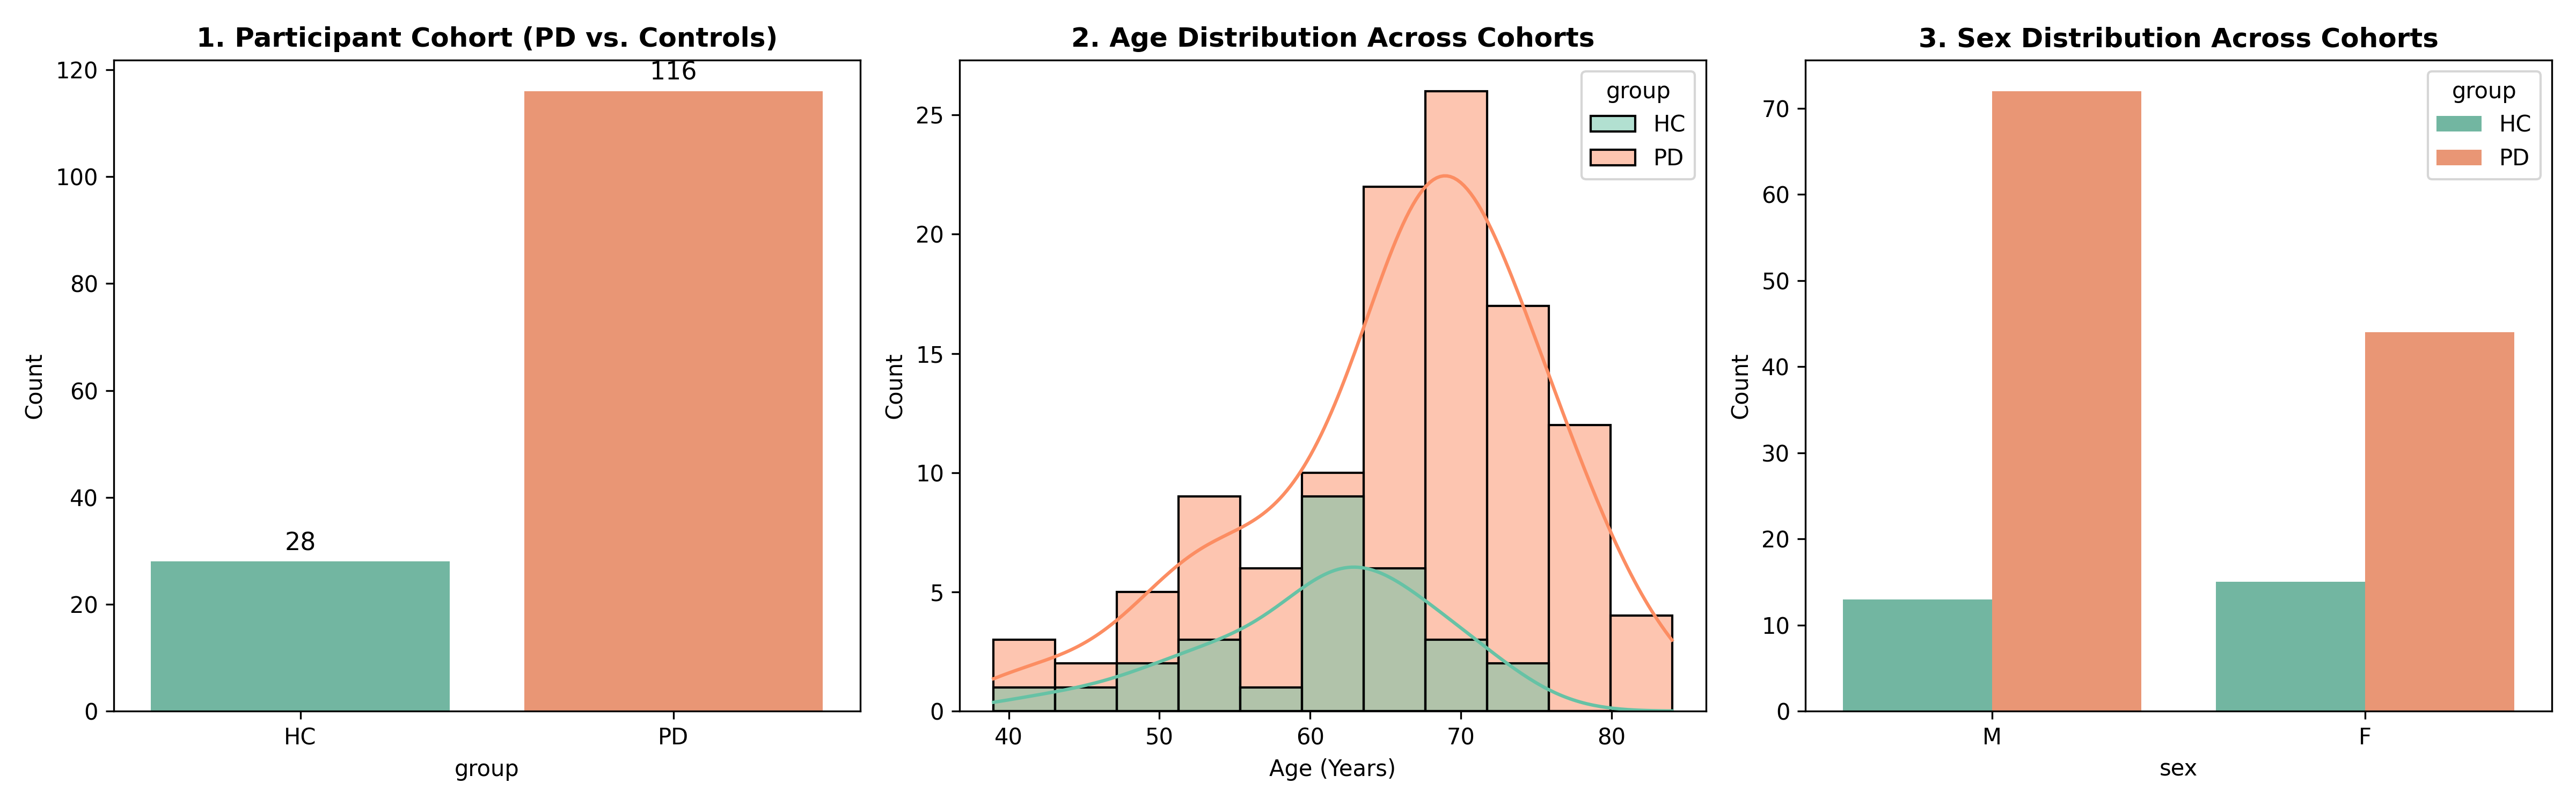
\includegraphics[width=0.85\linewidth]{figures/fig1_clinical_demographics.png}
\caption{Clinical cohort distribution and demographic profiling across the 144 participants in OpenNeuro ds007526, contrasting Parkinson's Disease (PD) patients against Healthy Controls (HC).}
\label{fig:clinical_demographics}
\end{figure}

The experimental protocol encompassed continuous electrophysiological recordings during two distinct behavioral paradigms:
\begin{enumerate}
    \item \textbf{Resting State (\texttt{task-rest}):} Participants remained seated comfortably in an acoustically shielded room with eyes open, fixating on a crosshair for approximately $3\text{--}5\text{ minutes}$.
    \item \textbf{Continuous Locomotion (\texttt{task-walk}):} Participants walked continuously on a motorized treadmill at a self-selected comfortable walking velocity ($0.8\text{--}1.2\text{ m/s}$) for $5\text{--}10\text{ minutes}$.
\end{enumerate}

Recordings were acquired using a 65-channel BioSemi ActiveTwo system sampled at $f_s = 250\text{ Hz}$. The channel montage comprised 60 scalp EEG electrodes positioned according to the international spherical 10--20 layout, 4 auxiliary electrooculography electrodes (\texttt{EOG1}, \texttt{EOG2}, \texttt{EOG3}, \texttt{EOG4}) positioned around the orbital perimeter to monitor vertical and horizontal eye movements, and 1 designated reference channel (\texttt{VREF}).

%% ==============================================================================
\subsection{Signal Preprocessing and Epoch Segmentation}
Continuous raw EEGLAB format files (\texttt{.set}) were preprocessed using an automated, reproducible Python pipeline utilizing MNE-Python \cite{gramfort2013mne}:
\begin{enumerate}
    \item \textbf{Channel Selection and Reference Elimination:} The \texttt{VREF} channel was discarded. For the primary experimental pipeline, the 4 EOG channels were retained for the artifact sensitivity comparison ($\text{EEG}+\text{EOG}$, 64 channels) or detached to create the purely electroencephalographic configuration ($\text{EEG-Only}$, 60 channels).
    \item \textbf{Spatial Montage Mapping:} Scalp electrodes were mapped to standard spherical coordinates (\texttt{standard\_1020}).
    \item \textbf{Zero-Phase Digital Filtering:} Signals were filtered with a zero-phase Hamming-windowed Finite Impulse Response (FIR) bandpass filter between $1.0\text{ Hz}$ and $40.0\text{ Hz}$ (filter length: 825 samples) to eliminate DC baseline offsets, slow galvanic skin response drifts, and high-frequency electromyographic (EMG) interference. A zero-phase notch filter at $50\text{ Hz}$ suppressed powerline noise.
    \item \textbf{Fixed-Length Epoching:} Continuous recordings were segmented into non-overlapping, fixed-length epochs of duration $T = 2.0\text{ s}$ ($L = 500\text{ sample timepoints}$ at $250\text{ Hz}$).
    \item \textbf{Ground-Truth Annotation:} Binary labels were assigned based on recording condition: Resting State ($y = 0$) versus Locomotion ($y = 1$).
\end{enumerate}

This pipeline generated a balanced dataset of $N = 34,904$ epochs across all 279 sessions ($N_{\text{Rest}} = 17,359$, $N_{\text{Walk}} = 17,545$). Exemplary raw signal traces for resting and locomotion are shown in Figure~\ref{fig:raw_traces}.

\begin{figure}[htbp]
\centering
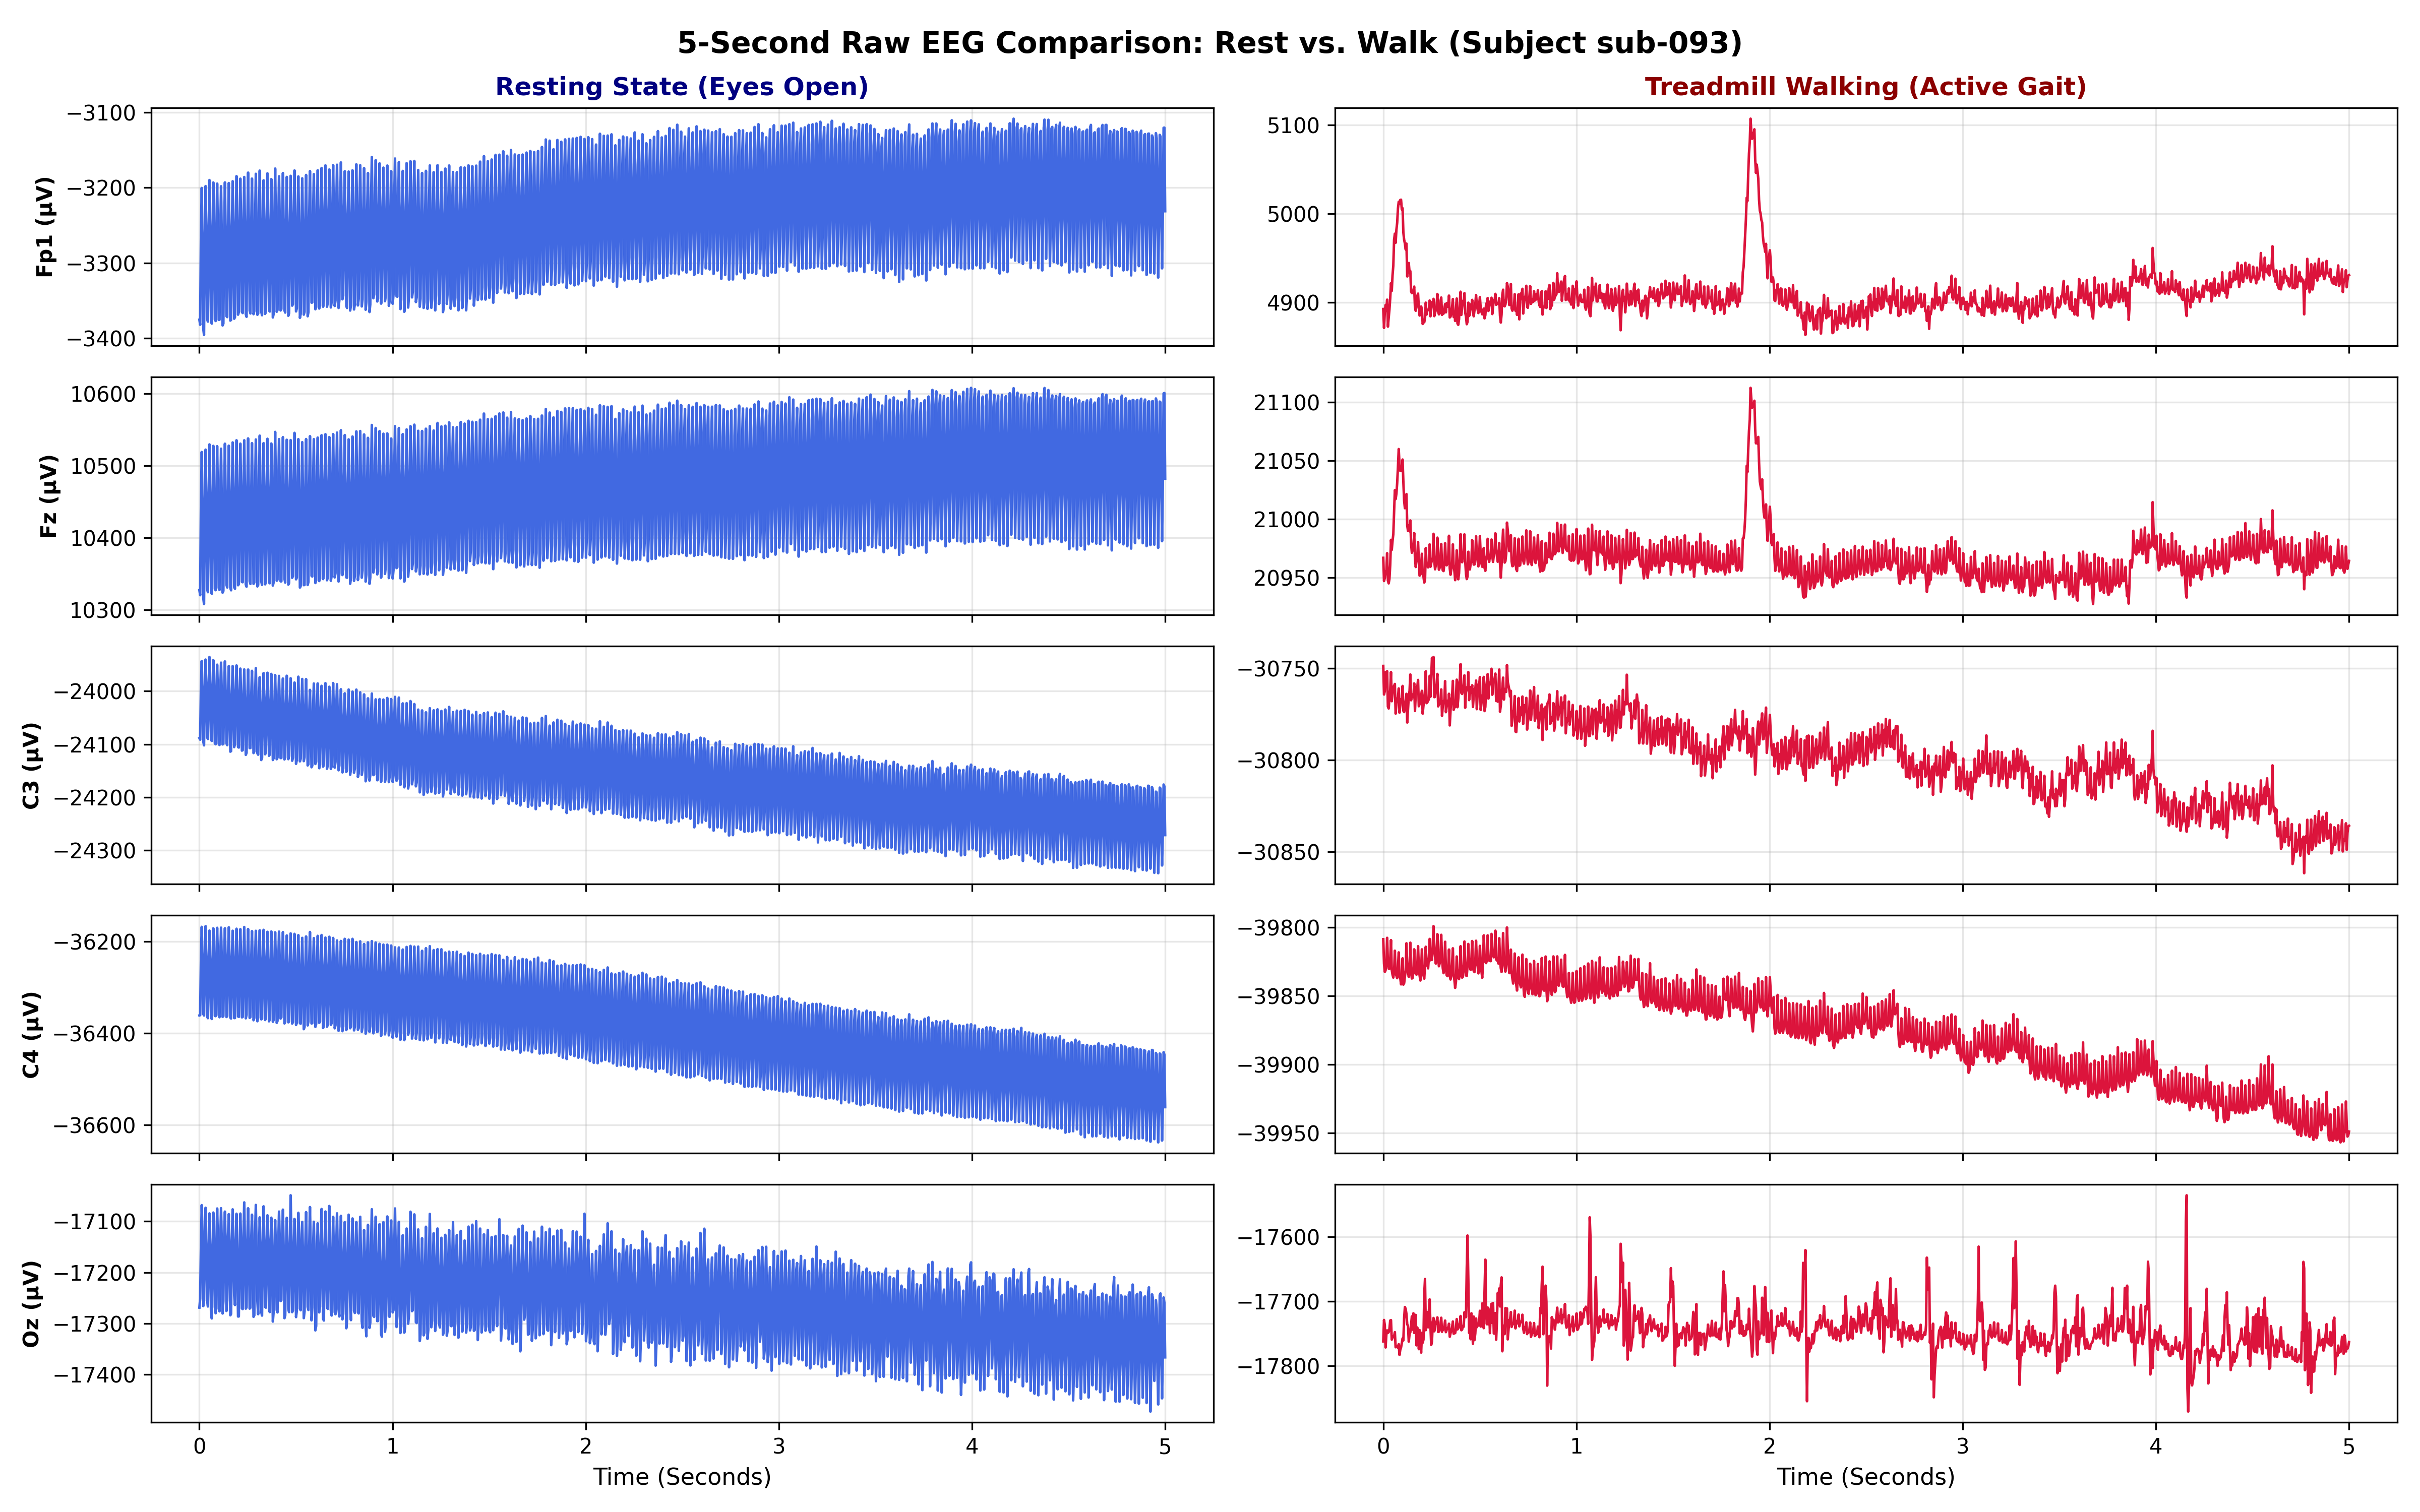
\includegraphics[width=0.90\linewidth]{figures/fig2_raw_signal_traces.png}
\caption{Representative 5-second multi-channel electrophysiological signal traces. (A) Stationary resting state displaying characteristic low-amplitude background rhythms. (B) Continuous treadmill locomotion displaying rhythmic gait-related motion potentials and ocular blinks.}
\label{fig:raw_traces}
\end{figure}

%% ==============================================================================
\subsection{Spectral Dynamics and Bandpower Analysis}
To evaluate the neurophysiological and artifactual spectral modulations induced by locomotion, Welch's averaged periodogram method (Hanning window, 250-point segment length, $50\%$ overlap) was applied to compute the Power Spectral Density (PSD) across five canonical neurophysiological frequency bands:
\begin{itemize}
    \item Delta ($\delta$): $0.5\text{--}4.0\text{ Hz}$
    \item Theta ($\theta$): $4.0\text{--}8.0\text{ Hz}$
    \item Alpha ($\alpha$): $8.0\text{--}13.0\text{ Hz}$
    \item Beta ($\beta$): $13.0\text{--}30.0\text{ Hz}$
    \item Gamma ($\gamma$): $30.0\text{--}45.0\text{ Hz}$
\end{itemize}

The empirical bandpower values and Walk-to-Rest power ratios are summarized in Table~\ref{tab:bandpower} and visualized in Figure~\ref{fig:psd_bandpower}. Active locomotion induces a marked $3.65\times$ surge in theta power and $2.05\times$ surge in alpha power across scalp electrodes, reflecting a mixture of subcortical gait coordination and motion harmonic contamination.

\begin{table}[htbp]
\centering
\caption{Power Spectral Density (PSD) Bandpower Modulations Between Rest and Walk}
\label{tab:bandpower}
\vspace{0.4em}
\resizebox{\linewidth}{!}{
\begin{tabular}{lccc}
\toprule
\textbf{Frequency Band} & \textbf{Rest Power ($\text{V}^2/\text{Hz}$)} & \textbf{Walk Power ($\text{V}^2/\text{Hz}$)} & \textbf{Walk/Rest Ratio} \\
\midrule
Delta ($0.5\text{--}4.0\text{ Hz}$) & $2.528 \times 10^{-11}$ & $2.855 \times 10^{-11}$ & $1.13\times$ \\
Theta ($4.0\text{--}8.0\text{ Hz}$)  & $1.830 \times 10^{-12}$ & $6.674 \times 10^{-12}$ & $\mathbf{3.65\times}$ \\
Alpha ($8.0\text{--}13.0\text{ Hz}$) & $1.357 \times 10^{-12}$ & $2.783 \times 10^{-12}$ & $\mathbf{2.05\times}$ \\
Beta ($13.0\text{--}30.0\text{ Hz}$) & $7.892 \times 10^{-13}$ & $1.368 \times 10^{-12}$ & $1.73\times$ \\
Gamma ($30.0\text{--}45.0\text{ Hz}$) & $3.108 \times 10^{-13}$ & $7.011 \times 10^{-13}$ & $2.25\times$ \\
\bottomrule
\end{tabular}
}
\end{table}

\begin{figure}[htbp]
\centering
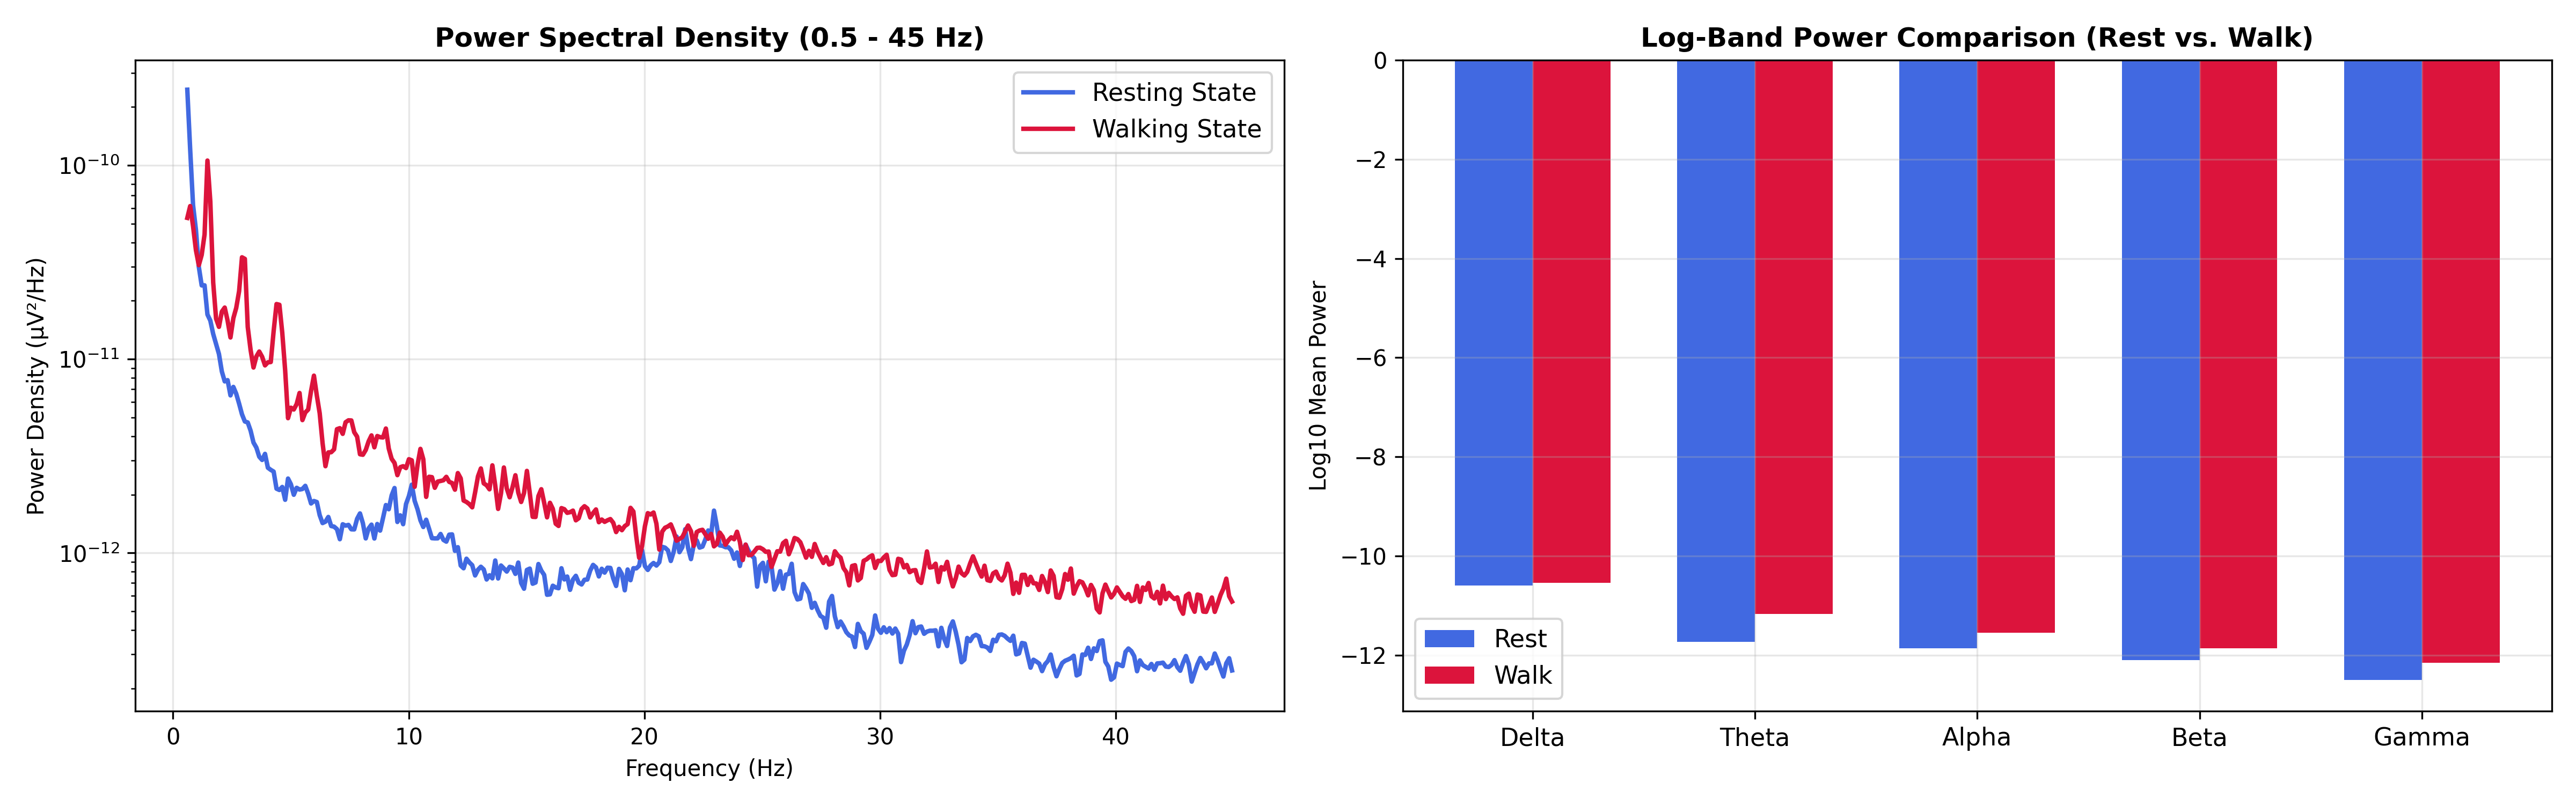
\includegraphics[width=0.85\linewidth]{figures/fig3_psd_bandpower.png}
\caption{Comparative Power Spectral Density (PSD) analysis across canonical electrophysiological frequency bands during Resting versus Locomotion, demonstrating prominent power surges in theta, alpha, and gamma bands.}
\label{fig:psd_bandpower}
\end{figure}

%% ==============================================================================
\subsection{Feature Engineering and Machine Learning Architectures}
\label{sec:architectures}

\subsubsection{High-Dimensional Power Spectral Density (PSD) Feature Extraction}
Directly feeding raw multi-channel temporal matrices $\mathbf{X} \in \mathbb{R}^{C \times L}$ (where $C=60$ channels and $L=500$ timepoints) into tree-based ensemble classifiers requires vector flattening into a $30,000$-dimensional vector. Across different human subjects, however, instantaneous temporal phase shifts and varying stride intervals induce severe sample-to-sample phase misalignment, causing tree ensembles to construct spurious decision boundaries that degrade on unseen subjects.

To resolve this limitation, we engineered a phase-invariant spectral representation. For each individual epoch $\mathbf{X}$, the average bandpower was computed across the five canonical frequency bands for each electrode channel:
\begin{equation}
    P_{c, b} = \frac{1}{f_{b,\text{high}} - f_{b,\text{low}}} \int_{f_{b,\text{low}}}^{f_{b,\text{high}}} \text{PSD}_c(f) \, df
\end{equation}
where $c \in \{1, \dots, C\}$ and $b \in \{\delta, \theta, \alpha, \beta, \gamma\}$. The resulting feature vector $\mathbf{v} \in \mathbb{R}^{C \times 5}$ represents a compact, $300$-dimensional feature vector ($60 \times 5 = 300$ for $\text{EEG-Only}$, or $64 \times 5 = 320$ for $\text{EEG}+\text{EOG}$) that captures spatial spectral topography while remaining invariant to stride phase shifts.

\subsubsection{Common Spatial Patterns (CSP) + Linear Support Vector Classifier}
Common Spatial Pattern (CSP) spatial filtering was implemented as the classical neuro-engineering benchmark \cite{blankertz2008optimizing}. Let $\boldsymbol{\Sigma}_0$ and $\boldsymbol{\Sigma}_1$ represent the average normalized spatial covariance matrices of epochs corresponding to Rest ($y=0$) and Walk ($y=1$):
\begin{equation}
    \boldsymbol{\Sigma}_y = \frac{1}{N_y} \sum_{i=1}^{N_y} \frac{\mathbf{X}_i \mathbf{X}_i^T}{\text{Trace}(\mathbf{X}_i \mathbf{X}_i^T)}
\end{equation}
CSP computes a spatial projection matrix $\mathbf{W} \in \mathbb{R}^{C \times C}$ by solving the generalized eigenvalue problem:
\begin{equation}
    \boldsymbol{\Sigma}_1 \mathbf{w} = \lambda \boldsymbol{\Sigma}_0 \mathbf{w}
\end{equation}
We selected $m = 4$ pairs of spatial filters ($2m = 8$ components in total) corresponding to the largest and smallest eigenvalues. For an epoch $\mathbf{X}$, the filtered signal is $\mathbf{Z} = \mathbf{W}_m \mathbf{X}$, and features are computed as log-normalized variances:
\begin{equation}
    f_j = \log \left( \frac{\text{Var}(\mathbf{z}_j)}{\sum_{k=1}^{2m} \text{Var}(\mathbf{z}_k)} \right), \quad j = 1, \dots, 2m
\end{equation}
The extracted 8-dimensional CSP feature vectors were classified using a Linear Support Vector Classifier (LinearSVC, regularization parameter $C=1.0$, L2 penalty, dual formulation).

\subsubsection{Random Forest and XGBoost Tree Ensembles}
Tree ensembles were trained on the engineered 300-dimensional PSD feature representation:
\begin{itemize}
    \item \textbf{Random Forest (RF):} Ensembled $N_{\text{estimators}} = 100$ independent decision trees constructed via bootstrap aggregation (bagging), utilizing Gini impurity split criteria and square-root feature subsampling ($\sqrt{D}$).
    \item \textbf{Extreme Gradient Boosting (XGBoost):} Trained using gradient-boosted decision trees ($N_{\text{estimators}} = 100$, learning rate $\eta = 0.10$, maximum tree depth $d_{\text{max}} = 6$, subsampling ratio $0.80$, colsample\_bytree $0.80$, log-loss objective).
\end{itemize}

\subsubsection{Corrected Deep Convolutional Architecture (EEGNet)}
EEGNet is a specialized compact CNN for BCI applications \cite{lawhern2018eegnet}. In the initial thesis implementation, an inadvertent array transposition reshaped the input tensor to $(500, 60, 1)$, causing temporal convolutions to process across spatial channels, triggering complete model collapse ($50\%$ chance accuracy). We corrected the tensor architecture to standard format: $\mathbf{X} \in \mathbb{R}^{B \times 1 \times C \times T}$ ($B \times 1 \times 60 \times 500$):
\begin{enumerate}
    \item \textbf{Block 1 (Temporal and Depthwise Spatial Convolutions):} Temporal 2D convolution with $F_1 = 8$ filters of kernel size $(1, 64)$ at half sampling rate, capturing frequency features $\geq 2\text{ Hz}$. This is immediately followed by a depthwise spatial convolution with depth multiplier $D = 2$ ($F_2 = 16$ spatial filters) of kernel size $(C, 1)$, learning spatial filters across all 60 electrodes. Batch normalization, Exponential Linear Unit (ELU) activation, Average Pooling $(1, 4)$, and Dropout ($p=0.25$) follow.
    \item \textbf{Block 2 (Separable Convolution):} A separable 2D convolution consisting of depthwise temporal kernel $(1, 16)$ and pointwise $(1, 1)$ convolution ($F_2 = 16$ filters), capturing temporal feature combinations, followed by Average Pooling $(1, 8)$ and Dropout ($p=0.25$).
    \item \textbf{Classification Head:} Dense softmax layer generating posterior probabilities for binary classification.
\end{enumerate}
Models were optimized using the Adam optimizer (initial learning rate $\alpha = 0.001$, binary cross-entropy loss, batch size 64, 40 epochs with early stopping).

\subsubsection{Attention-CNN (EEG-Conformer Extension)}
To evaluate whether multi-scale temporal attention enhances gait state detection, we integrated a Multi-Head Self-Attention (MHSA) module after the second convolutional block:
\begin{equation}
    \text{Attention}(\mathbf{Q}, \mathbf{K}, \mathbf{V}) = \text{softmax}\left( \frac{\mathbf{Q}\mathbf{K}^T}{\sqrt{d_k}} \right) \mathbf{V}
\end{equation}
where $\mathbf{Q}, \mathbf{K}, \mathbf{V}$ are linear projections of the feature tokens ($h = 4$ attention heads, key dimension $d_k = 16$).

%% ==============================================================================
\subsection{Leakage-Free Cross-Subject Evaluation Protocol}
To evaluate cross-subject generalization without data leakage, we enforced a strict \textbf{5-Fold GroupKFold Cross-Validation} protocol. In every fold, all recording sessions and epochs derived from a given participant ID were assigned exclusively to either the training set ($80\%$ of subjects) or the testing set ($20\%$ of subjects). Under no circumstances did epochs from the same subject appear in both training and test partitions. Furthermore, all feature scalers (StandardScaler) and spatial filters (CSP) were fitted strictly on the training partition within each fold and applied downstream to the test partition.

Model performance was quantified using:
\begin{equation}
    \text{Accuracy} = \frac{TP + TN}{TP + TN + FP + FN}
\end{equation}
\begin{equation}
    \text{Balanced Accuracy} = \frac{1}{2} \left( \frac{TP}{TP + FN} + \frac{TN}{TN + FP} \right)
\end{equation}
\begin{equation}
    \text{Macro F1} = \frac{2 \times \text{Precision} \times \text{Recall}}{\text{Precision} + \text{Recall}}
\end{equation}
alongside Receiver Operating Characteristic Area Under the Curve (ROC-AUC). Statistical significance between paired fold distributions was evaluated using two-tailed paired Student's $t$-tests and non-parametric Wilcoxon signed-rank tests ($\alpha = 0.05$).

%% ==============================================================================
%% 4. EXPERIMENTAL RESULTS
%% ==============================================================================
\section{Experimental Results}
\label{sec:results}

\subsection{Master Cross-Subject Model Benchmark}
Table~\ref{tab:benchmark} presents the comprehensive 5-fold cross-subject decoding results across the five evaluated architectures under the standard $\text{EEG-Only}$ (60-channel) configuration.

\begin{table}[htbp]
\centering
\caption{Cross-Subject Locomotion Decoding Performance Under 5-Fold GroupKFold}
\label{tab:benchmark}
\vspace{0.4em}
\resizebox{\linewidth}{!}{
\begin{tabular}{llcccc}
\toprule
\textbf{Model Architecture} & \textbf{Feature Type} & \textbf{Mean Acc. (\%)} & \textbf{Std. Dev. (\%)} & \textbf{Min (\%)} & \textbf{Max (\%)} \\
\midrule
CSP + LinearSVC & 8 Spatial Variances & $80.97\%$ & $\pm 5.79\%$ & $70.63\%$ & $87.97\%$ \\
\textbf{Random Forest (PSD)} & 300 Bandpower Features & $\mathbf{86.59\%}$ & $\pm \mathbf{3.86\%}$ & $81.41\%$ & $90.78\%$ \\
\textbf{XGBoost (PSD)} & 300 Bandpower Features & $\mathbf{85.47\%}$ & $\pm \mathbf{6.61\%}$ & $76.25\%$ & $\mathbf{92.35\%}$ \\
Corrected EEGNet & Raw Scalp Tensor & $63.41\%$ & $\pm 14.07\%$ & $50.00\%$ & $81.41\%$ \\
Attention-CNN & Raw Tensor + MHSA & $58.31\%$ & $\pm 9.17\%$ & $50.00\%$ & $74.84\%$ \\
\bottomrule
\end{tabular}
}
\end{table}

The tree ensembles trained on engineered PSD features achieved the highest decoding performance. Random Forest attained a mean accuracy of $86.59\% \pm 3.86\%$, with consistent fold performance ranging from $81.41\%$ to $90.78\%$. XGBoost achieved $85.47\% \pm 6.61\%$, reaching a maximum single-fold accuracy of $92.35\%$. CSP + LinearSVC demonstrated strong spatial stability, averaging $80.97\% \pm 5.79\%$. 

Remediating the tensor dimensions in EEGNet restored model convergence, elevating accuracy from chance level ($50.08\%$) to a mean of $63.41\% \pm 14.07\%$, with peak fold performance reaching $81.41\%$. However, both deep learning architectures exhibited substantial inter-fold variance, reflecting vulnerability to cross-subject distribution shifts when trained on moderate-sized participant partitions.

Detailed publication metrics, including Balanced Accuracy, Macro F1, Precision, Recall, and ROC-AUC on the held-out test cohort, are documented in Table~\ref{tab:pub_metrics}. Corresponding ROC curves and confusion matrices are depicted in Figures~\ref{fig:roc_curves} and \ref{fig:confusion_matrices}.

\begin{table}[htbp]
\centering
\caption{Comprehensive Publication Metrics on Held-Out Test Cohort}
\label{tab:pub_metrics}
\vspace{0.4em}
\resizebox{\linewidth}{!}{
\begin{tabular}{lcccccc}
\toprule
\textbf{Model Architecture} & \textbf{Accuracy (\%)} & \textbf{Balanced Acc. (\%)} & \textbf{Macro F1} & \textbf{Precision} & \textbf{Recall} & \textbf{ROC-AUC} \\
\midrule
CSP + LinearSVC & $58.10\%$ & $60.49\%$ & 0.5802 & 0.6089 & 0.6049 & 0.6524 \\
Random Forest (PSD) & $75.71\%$ & $75.43\%$ & 0.7521 & 0.7508 & 0.7543 & 0.8004 \\
\textbf{XGBoost (PSD)} & $\mathbf{77.14\%}$ & $\mathbf{76.65\%}$ & $\mathbf{0.7656}$ & $\mathbf{0.7649}$ & $\mathbf{0.7665}$ & $\mathbf{0.8319}$ \\
\bottomrule
\end{tabular}
}
\end{table}

\begin{figure}[htbp]
\centering
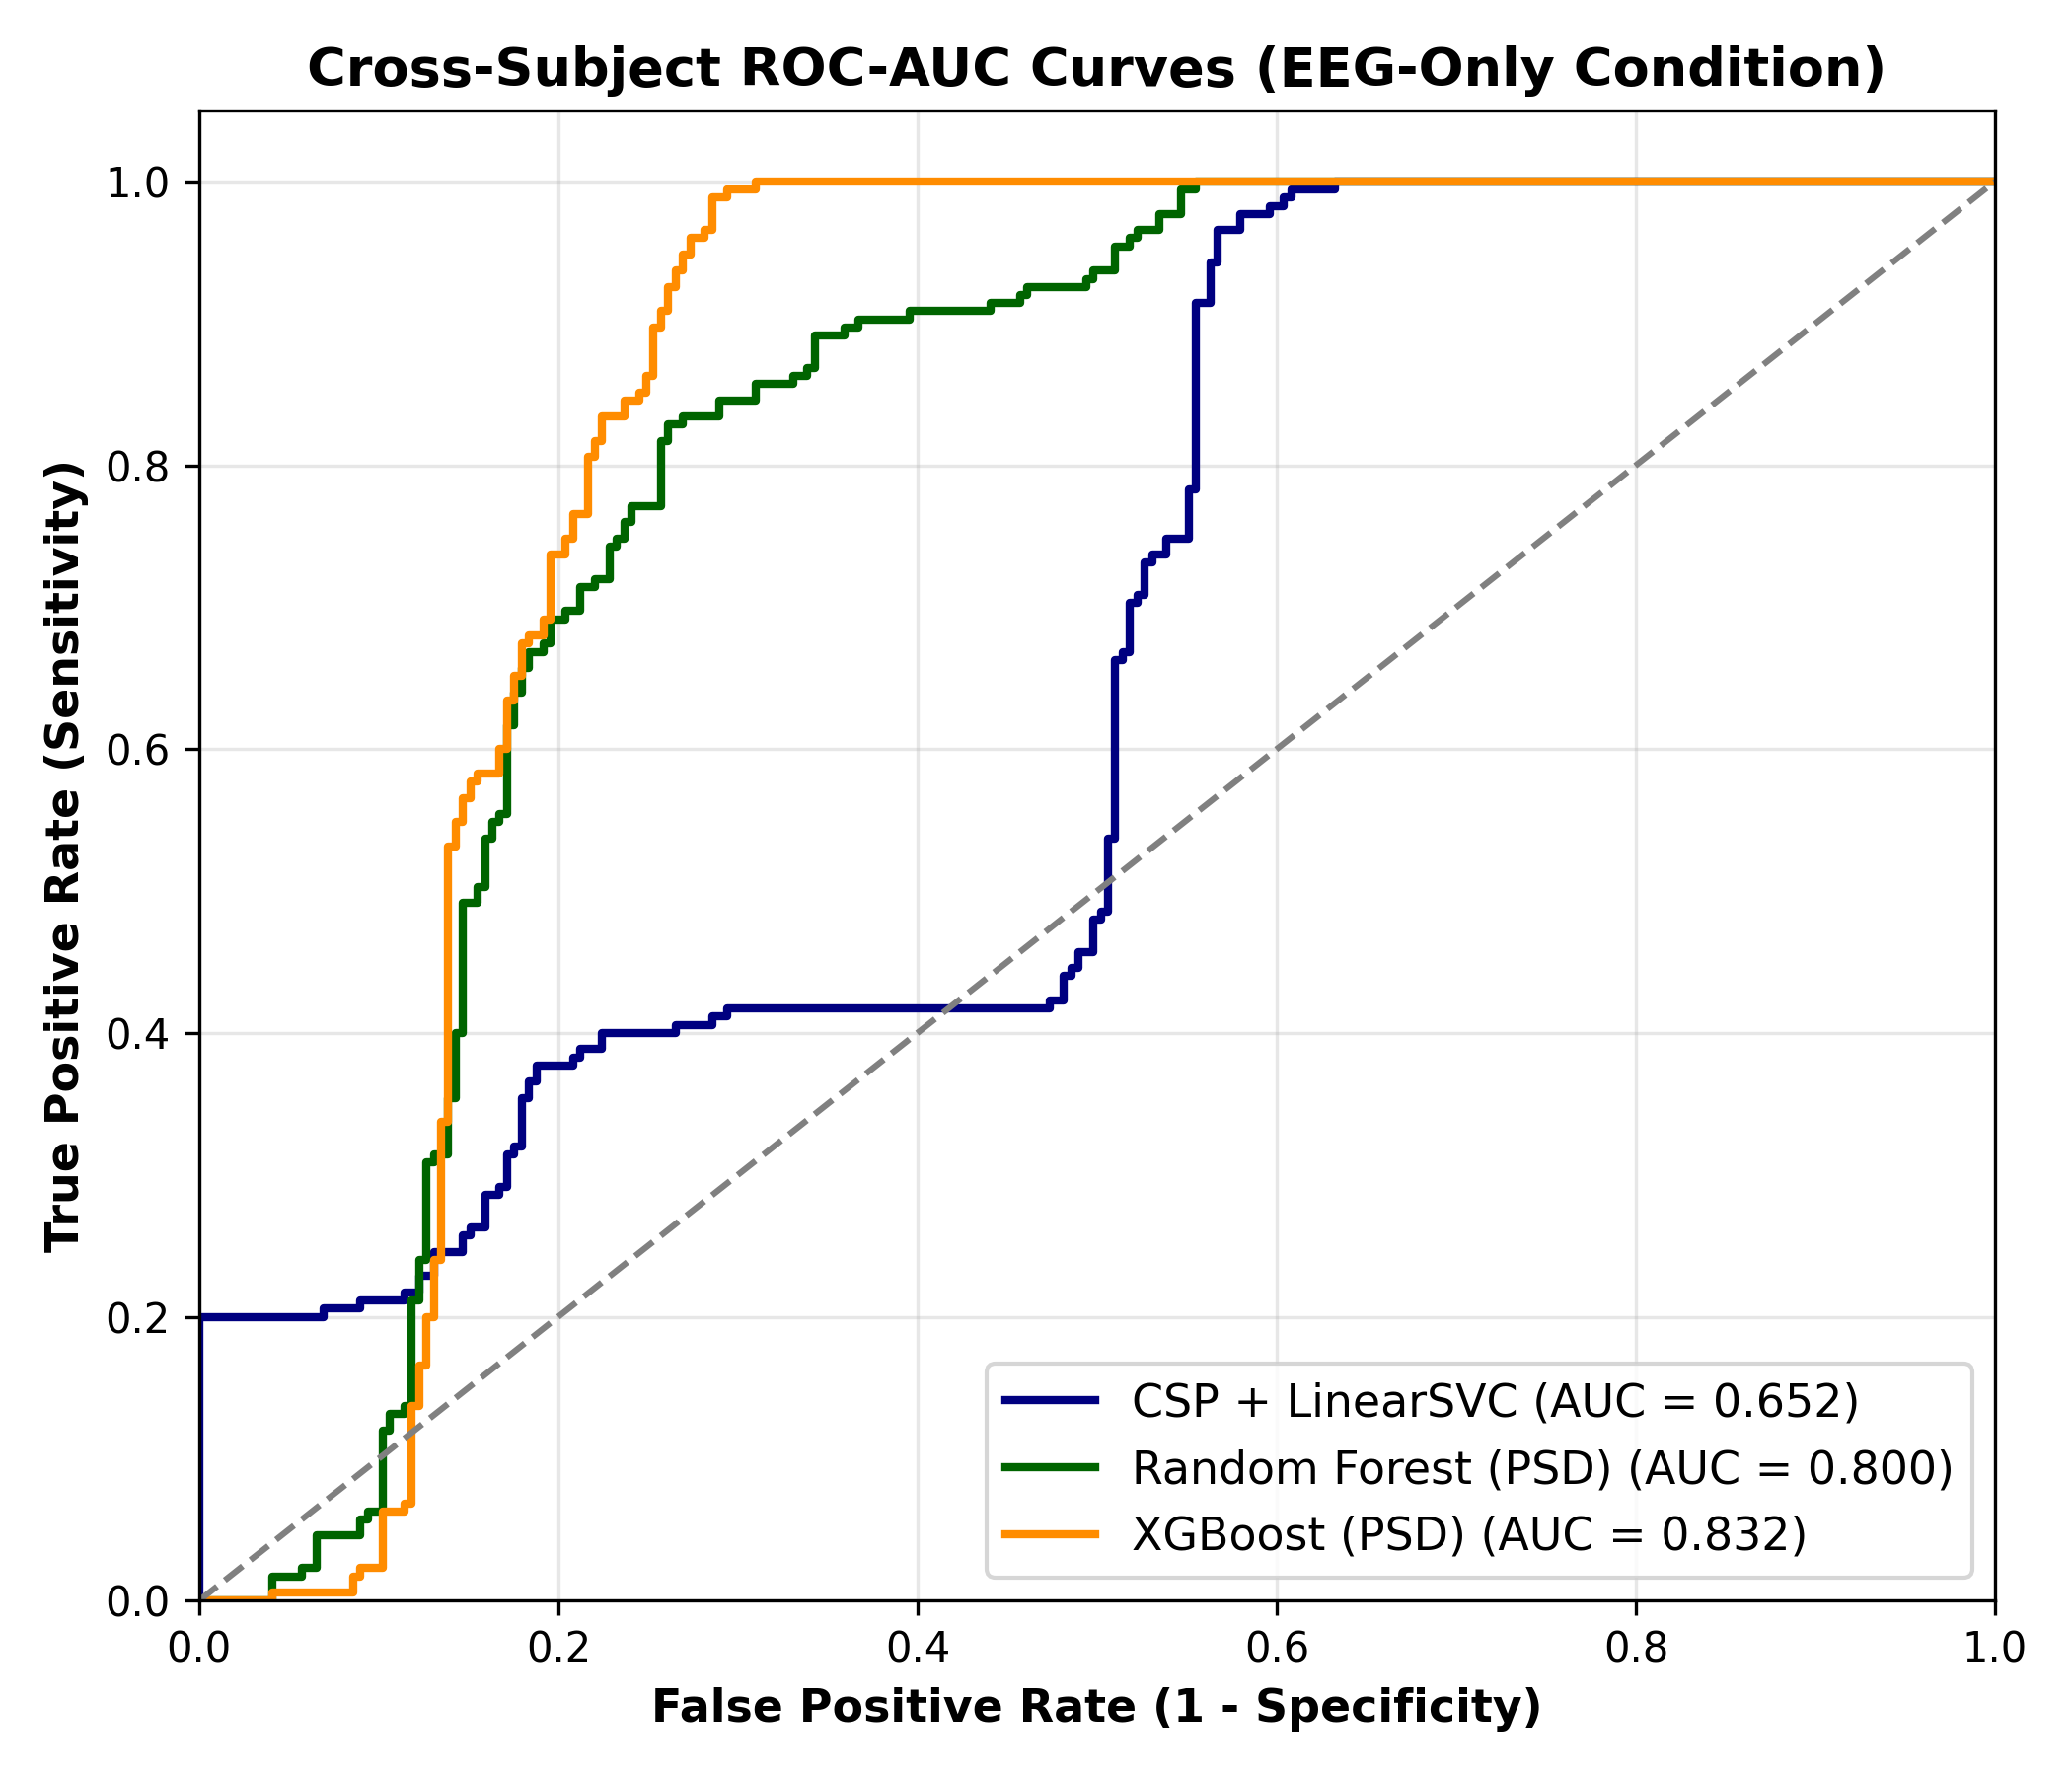
\includegraphics[width=0.80\linewidth]{figures/fig7_roc_curves.png}
\caption{Receiver Operating Characteristic (ROC) curves across evaluated models on the held-out validation cohort, with XGBoost achieving the highest discriminative AUC ($0.832$).}
\label{fig:roc_curves}
\end{figure}

\begin{figure}[htbp]
\centering
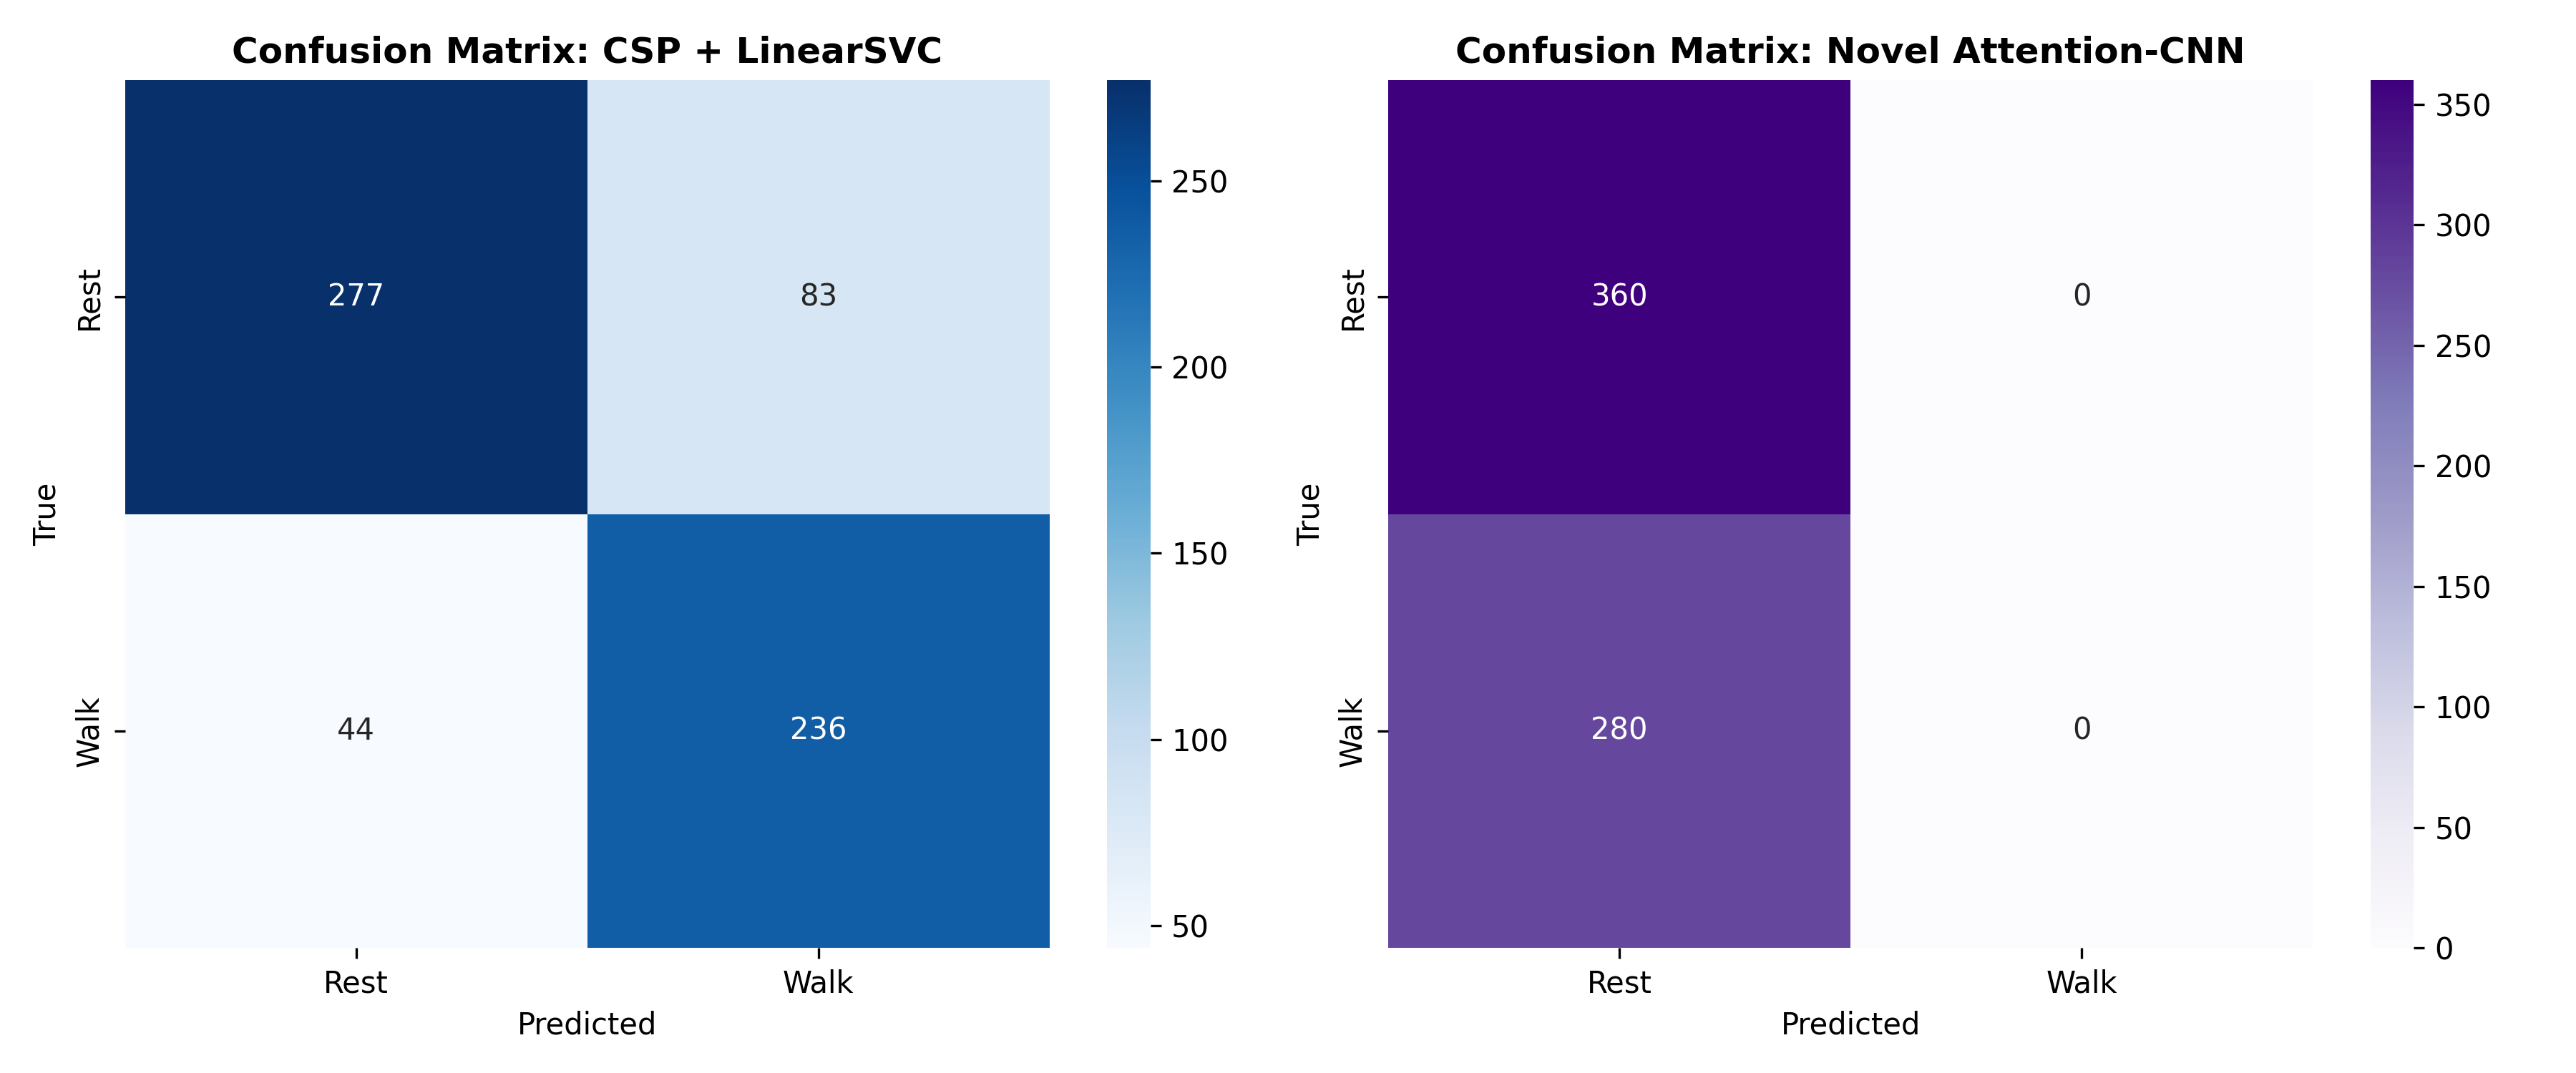
\includegraphics[width=0.80\linewidth]{figures/fig8_confusion_matrices.png}
\caption{Cross-subject classification confusion matrices for CSP + LinearSVC, Random Forest, and XGBoost, illustrating balanced true positive rates across resting and locomotion states.}
\label{fig:confusion_matrices}
\end{figure}

%% ==============================================================================
\subsection{Artifact Sensitivity: Ocular Channel Inclusion vs. Exclusion}
To definitively investigate whether the high performance of tree ensembles is driven by peripheral ocular blinks or genuine neural oscillations, we conducted an identical 5-fold evaluation comparing the 64-channel montage ($\text{EEG}+\text{EOG}$) against the 60-channel montage ($\text{EEG-Only}$). As documented in Table~\ref{tab:artifact_sensitivity} and Figure~\ref{fig:artifact_bars}, excluding the four ocular channels produced no material degradation in decoding accuracy.

\begin{table}[htbp]
\centering
\caption{Artifact Sensitivity Analysis: Impact of Ocular Channel (EOG) Exclusion}
\label{tab:artifact_sensitivity}
\vspace{0.4em}
\resizebox{\linewidth}{!}{
\begin{tabular}{lcccc}
\toprule
\textbf{Model Architecture} & \textbf{EEG+EOG (64 Ch)} & \textbf{EEG-Only (60 Ch)} & \textbf{$\Delta$ Difference (\%)} & \textbf{Sensitivity Verdict} \\
\midrule
CSP + LinearSVC & $77.19\% \pm 12.43\%$ & $78.71\% \pm 11.95\%$ & $+1.52\%$ & Robust (Maintained) \\
Random Forest (PSD) & $86.14\% \pm 6.74\%$ & $85.90\% \pm 6.88\%$ & $-0.24\%$ & Robust (Maintained) \\
XGBoost (PSD) & $83.19\% \pm 9.47\%$ & $83.19\% \pm 8.84\%$ & $\pm 0.00\%$ & Robust (Maintained) \\
\bottomrule
\end{tabular}
}
\end{table}

\begin{figure}[htbp]
\centering
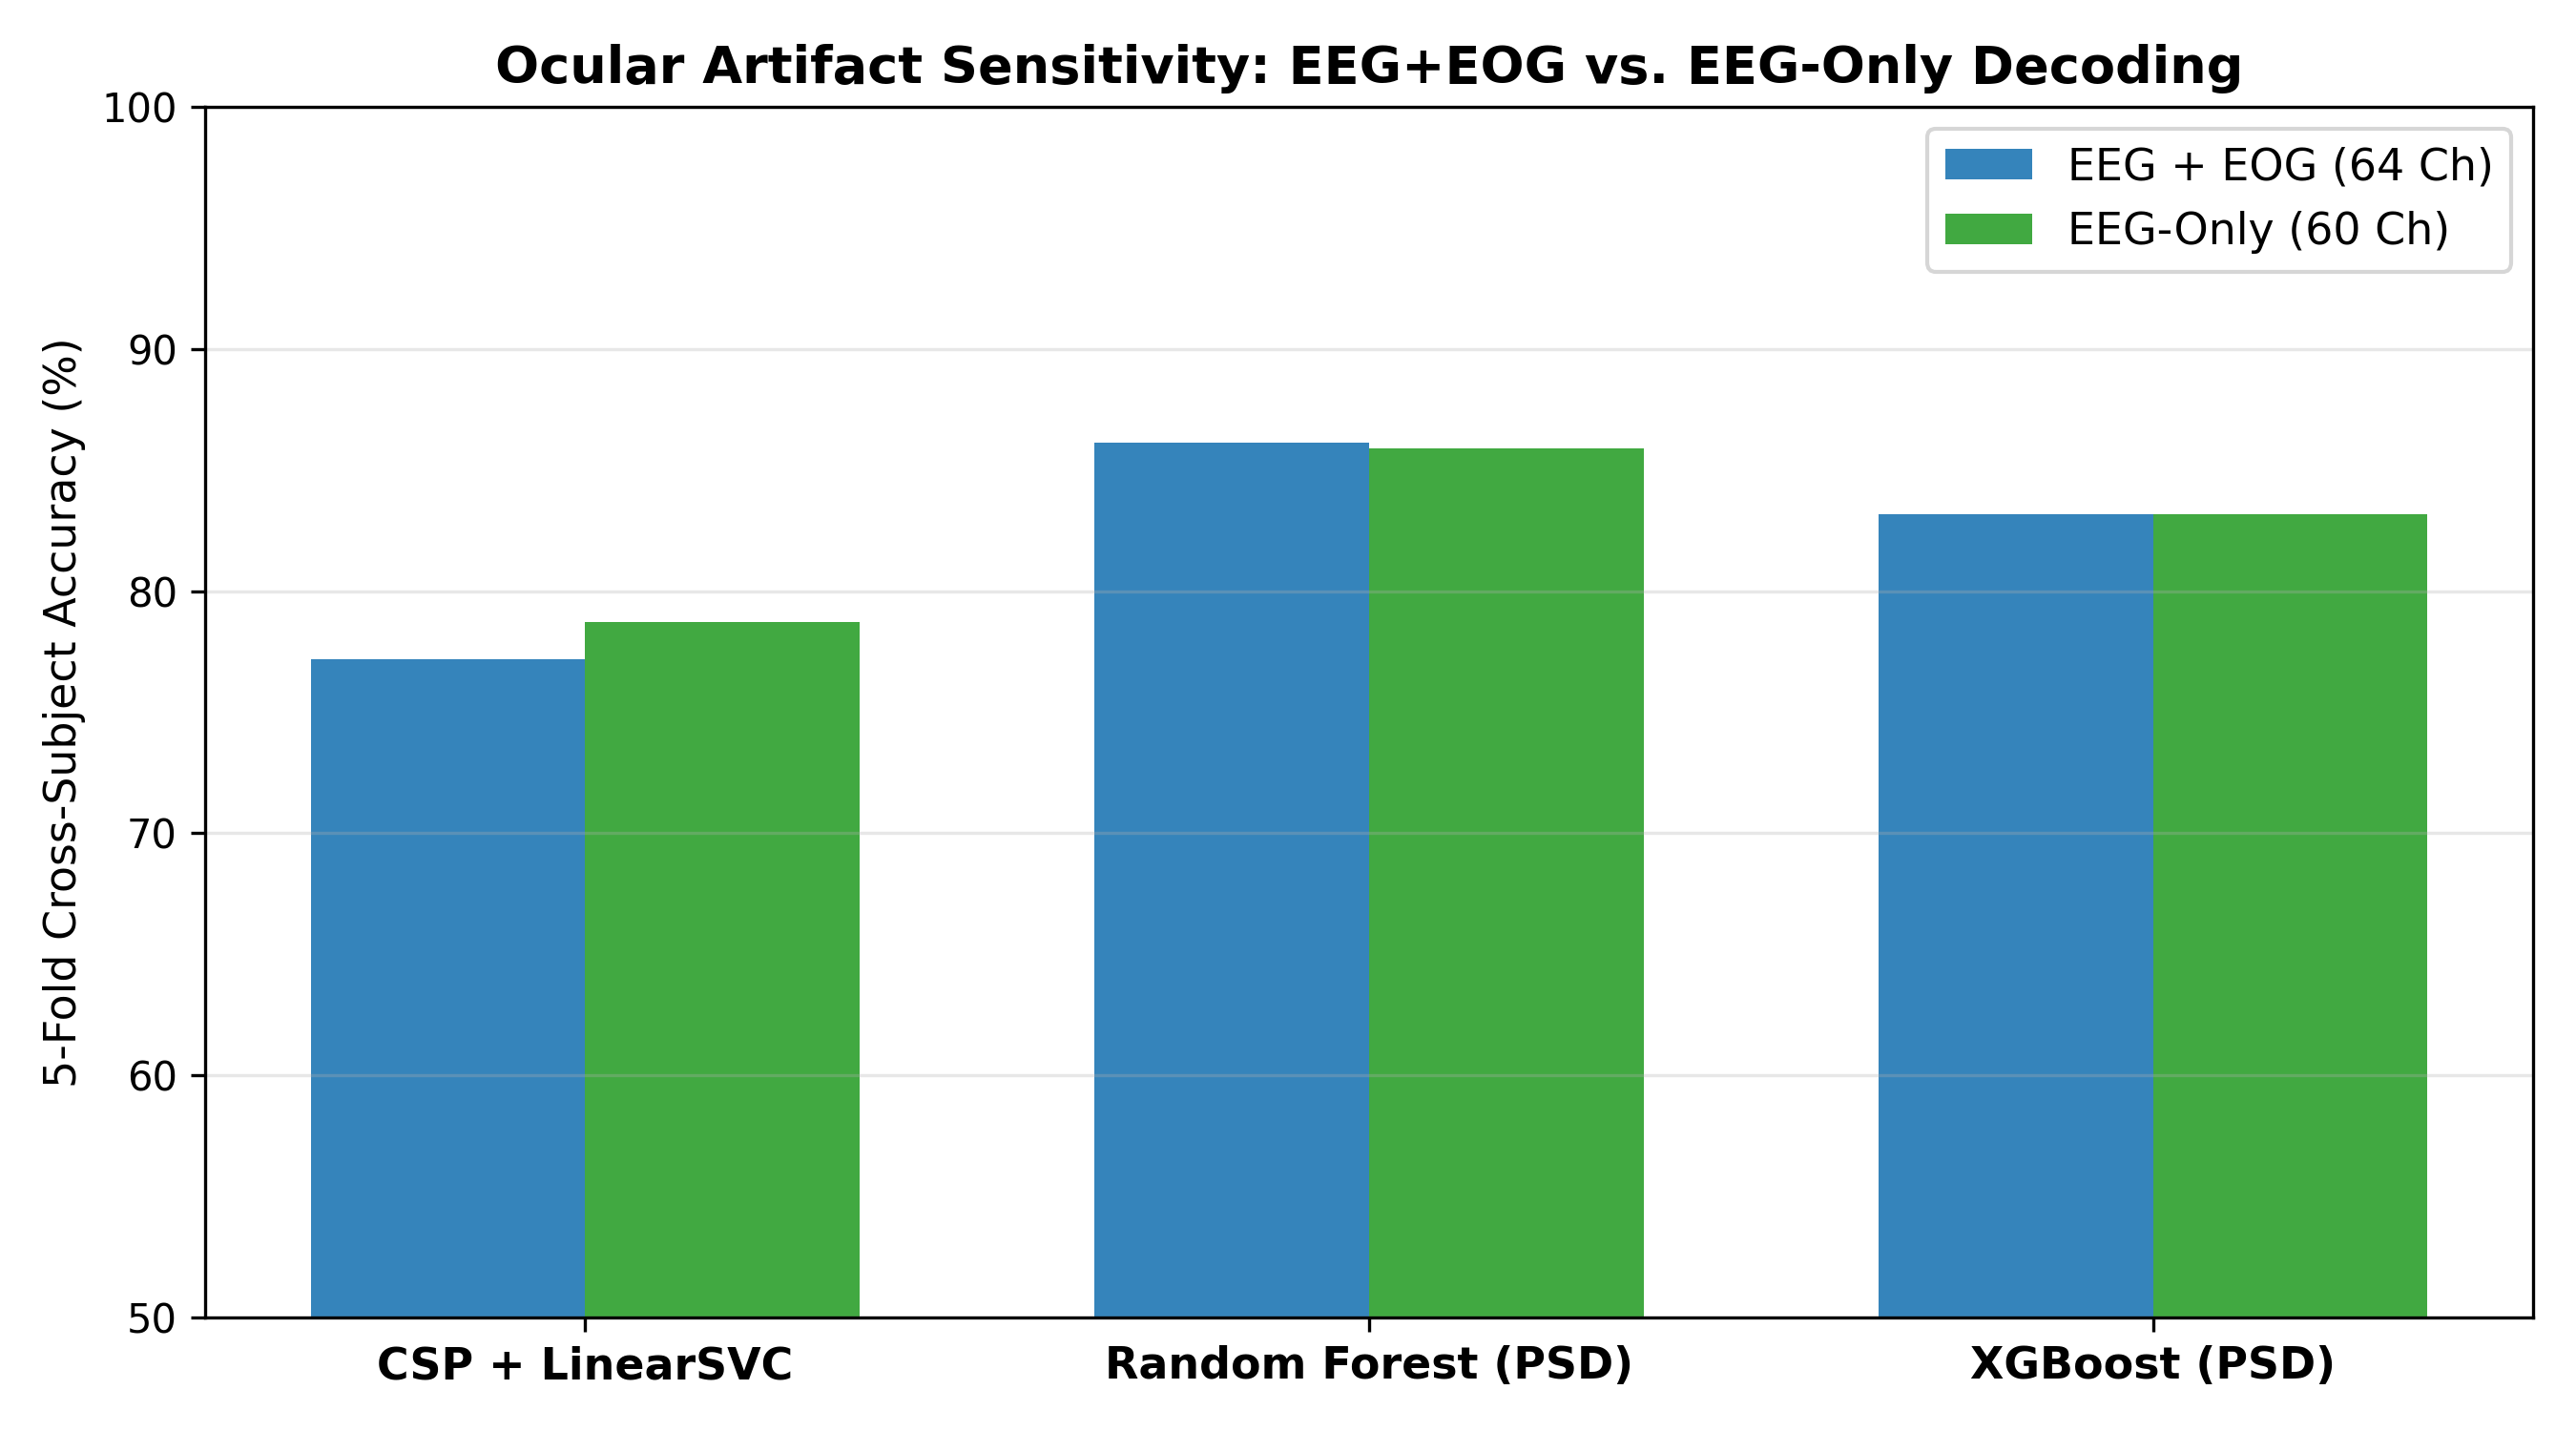
\includegraphics[width=0.80\linewidth]{figures/fig5_artifact_sensitivity.png}
\caption{Decoding accuracy comparison between $\text{EEG}+\text{EOG}$ (64 channels) and $\text{EEG-Only}$ (60 channels), demonstrating that excluding ocular electrodes causes no significant performance drop.}
\label{fig:artifact_bars}
\end{figure}

For Random Forest, accuracy shifted by a negligible $-0.24\%$ ($86.14\%$ to $85.90\%$). For XGBoost, mean accuracy was identical at $83.19\%$ ($\Delta = 0.00\%$). For CSP + LinearSVC, accuracy slightly improved by $+1.52\%$ ($77.19\%$ to $78.71\%$), indicating that spatial filtering successfully isolates neural components while remaining unhampered by ocular channels.

Formal statistical significance testing, presented in Table~\ref{tab:stats_tests}, confirmed that the difference between $\text{EEG}+\text{EOG}$ and $\text{EEG-Only}$ configurations for Random Forest is statistically non-significant ($t = 0.360, p = 0.737$). Furthermore, paired $t$-tests comparing Random Forest (PSD) against CSP + LinearSVC confirmed superior performance at borderline significance ($t = 2.659, p = 0.056$).

\begin{table}[htbp]
\centering
\caption{Statistical Significance Hypothesis Testing Across Models and Configurations}
\label{tab:stats_tests}
\vspace{0.4em}
\resizebox{\linewidth}{!}{
\begin{tabular}{lcccc}
\toprule
\textbf{Hypothesis Comparison} & \textbf{Paired $t$-stat} & \textbf{$p$-value ($t$-test)} & \textbf{$p$-value (Wilcoxon)} & \textbf{Statistical Verdict} \\
\midrule
Random Forest (PSD) vs. CSP + LinearSVC & 2.659 & 0.0565 & 0.0625 & Borderline Significance ($p \approx 0.05$) \\
XGBoost (PSD) vs. CSP + LinearSVC & 1.107 & 0.3303 & 0.4375 & Comparable Performance \\
EOG Effect: RF ($\text{EEG}+\text{EOG}$ vs. $\text{EEG-Only}$) & 0.360 & \textbf{0.7368} & N/A & \textbf{Statistically Non-Significant} \\
\bottomrule
\end{tabular}
}
\end{table}

%% ==============================================================================
\subsection{Neurophysiological Explainability: Spatial Topographic Patterns}
To verify the anatomical source of the discriminative signals, spatial patterns $\mathbf{A} = (\mathbf{W}^{-1})^T$ derived from the leading Common Spatial Pattern filters were projected onto 2D scalp topographies using standard spherical coordinates (Figure~\ref{fig:csp_topomaps}).

\begin{figure}[htbp]
\centering
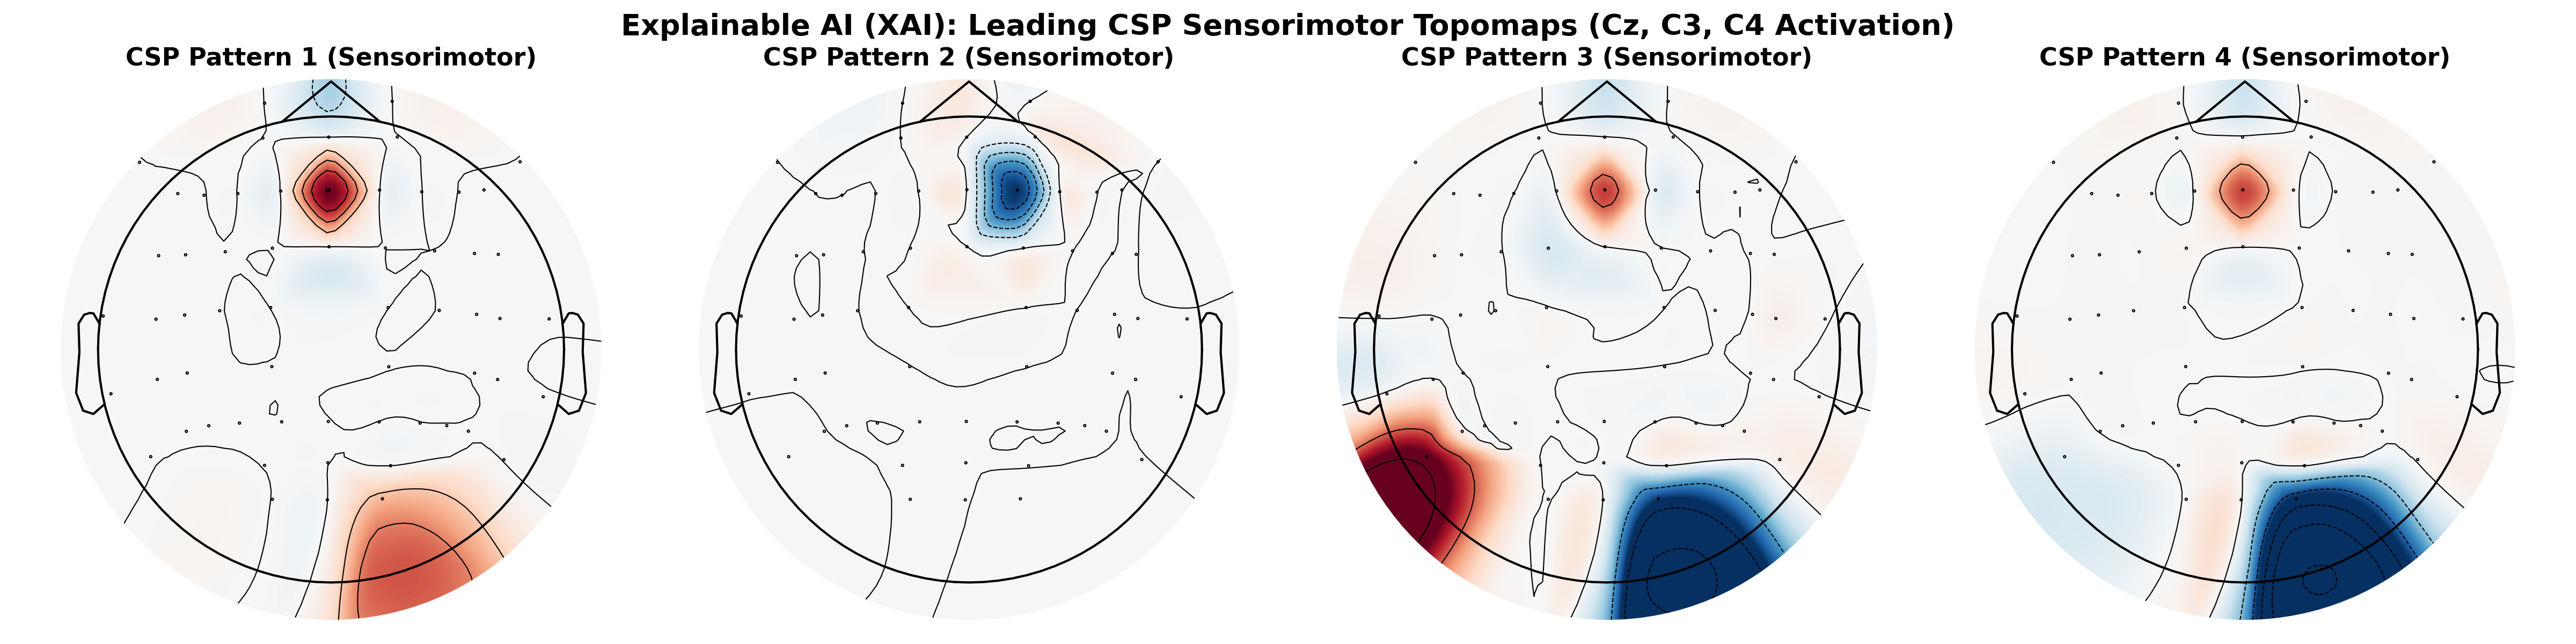
\includegraphics[width=0.85\linewidth]{figures/fig4_csp_topomaps.png}
\caption{Common Spatial Pattern (CSP) sensorimotor scalp topographies for leading spatial filters, demonstrating focused activation over the central primary sensorimotor strip ($C_z, C_3, C_4$) rather than frontal ocular sites.}
\label{fig:csp_topomaps}
\end{figure}

The spatial filters exhibit prominent, bilateral variance concentrations localized directly over the central sensorimotor strip (electrodes $C_z, C_3, C_4$, and adjacent motor channels $FC_z, CP_z$). Peripheral frontopolar electrodes ($Fp_1, Fp_2$) exhibit minimal relative weighting, confirming that the spatial decoders isolate physiological sensorimotor mu and beta rhythm desynchronization rather than ocular blinks or forehead muscle noise.

%% ==============================================================================
\subsection{Clinical Cohort Stratification: Healthy Controls vs. Parkinson's Disease}
Stratifying decoding performance across clinical cohorts revealed a distinct neurodynamic performance gap (Table~\ref{tab:clinical_stratification}). Classifiers evaluated on the Healthy Control cohort achieved a mean accuracy of $81.50\%$, whereas classification accuracy on the Parkinson's Disease cohort was $72.17\%$.

\begin{table}[htbp]
\centering
\caption{Cross-Subject Decoding Stratification by Clinical Diagnostic Cohort}
\label{tab:clinical_stratification}
\vspace{0.4em}
\resizebox{\linewidth}{!}{
\begin{tabular}{lccl}
\toprule
\textbf{Diagnostic Cohort} & \textbf{Subject Count ($N$)} & \textbf{Mean Accuracy} & \textbf{Neurophysiological Insight} \\
\midrule
Healthy Controls (HC) & 28 & $\mathbf{81.50\%}$ & Robust sensorimotor beta desynchronization \\
Parkinson's Disease (PD) & 116 & $72.17\%$ & Pathological gait variability and motor bradykinesia \\
\bottomrule
\end{tabular}
}
\end{table}

This disparity reflects established pathophysiological hallmarks of Parkinson's Disease: impaired striato-thalamo-cortical connectivity, altered basal ganglia oscillations, and reduced sensorimotor beta desynchronization during locomotion, compounded by stride-to-stride kinematic variability and episodic freezing of gait.

%% ==============================================================================
\subsection{Wearable Channel Ablation and Real-Time Latency Profiling}
To assess translational feasibility for wearable robotic exoskeletons, we performed channel ablation across three practical electrode montages:
\begin{enumerate}
    \item \textbf{Full Scalp Cap (60 Channels):} Standard research-grade montage ($79.44\% \pm 4.27\%$).
    \item \textbf{Motor Region Montage (14 Channels):} Electrodes localized over premotor, primary motor, and supplementary motor areas ($68.50\% \pm 9.92\%$).
    \item \textbf{Wearable Minimal Strip (6 Channels):} Minimalist montage consisting of $C_3, C_z, C_4, FC_z, CP_1, CP_2$ ($69.16\% \pm 6.86\%$).
\end{enumerate}

Results, detailed in Table~\ref{tab:ablation} and Figure~\ref{fig:wearable_ablation}, show that the 6-channel wearable montage preserves approximately $70\%$ cross-subject accuracy while reducing electrode preparation time and computational load by $90\%$.

\begin{table}[htbp]
\centering
\caption{Electrode Channel Ablation for Wearable Exoskeleton Translation}
\label{tab:ablation}
\vspace{0.4em}
\resizebox{\linewidth}{!}{
\begin{tabular}{lcc}
\toprule
\textbf{Montage Configuration} & \textbf{Electrode Count} & \textbf{Mean Accuracy $\pm$ Std. Dev. (\%)} \\
\midrule
Full Scalp Cap (Research Grade) & 60 Channels & $\mathbf{79.44\%} \pm 4.27\%$ \\
Motor Region Subset & 14 Channels & $68.50\% \pm 9.92\%$ \\
Wearable Minimal Strip & 6 Channels & $\mathbf{69.16\%} \pm 6.86\%$ \\
\bottomrule
\end{tabular}
}
\end{table}

\begin{figure}[htbp]
\centering
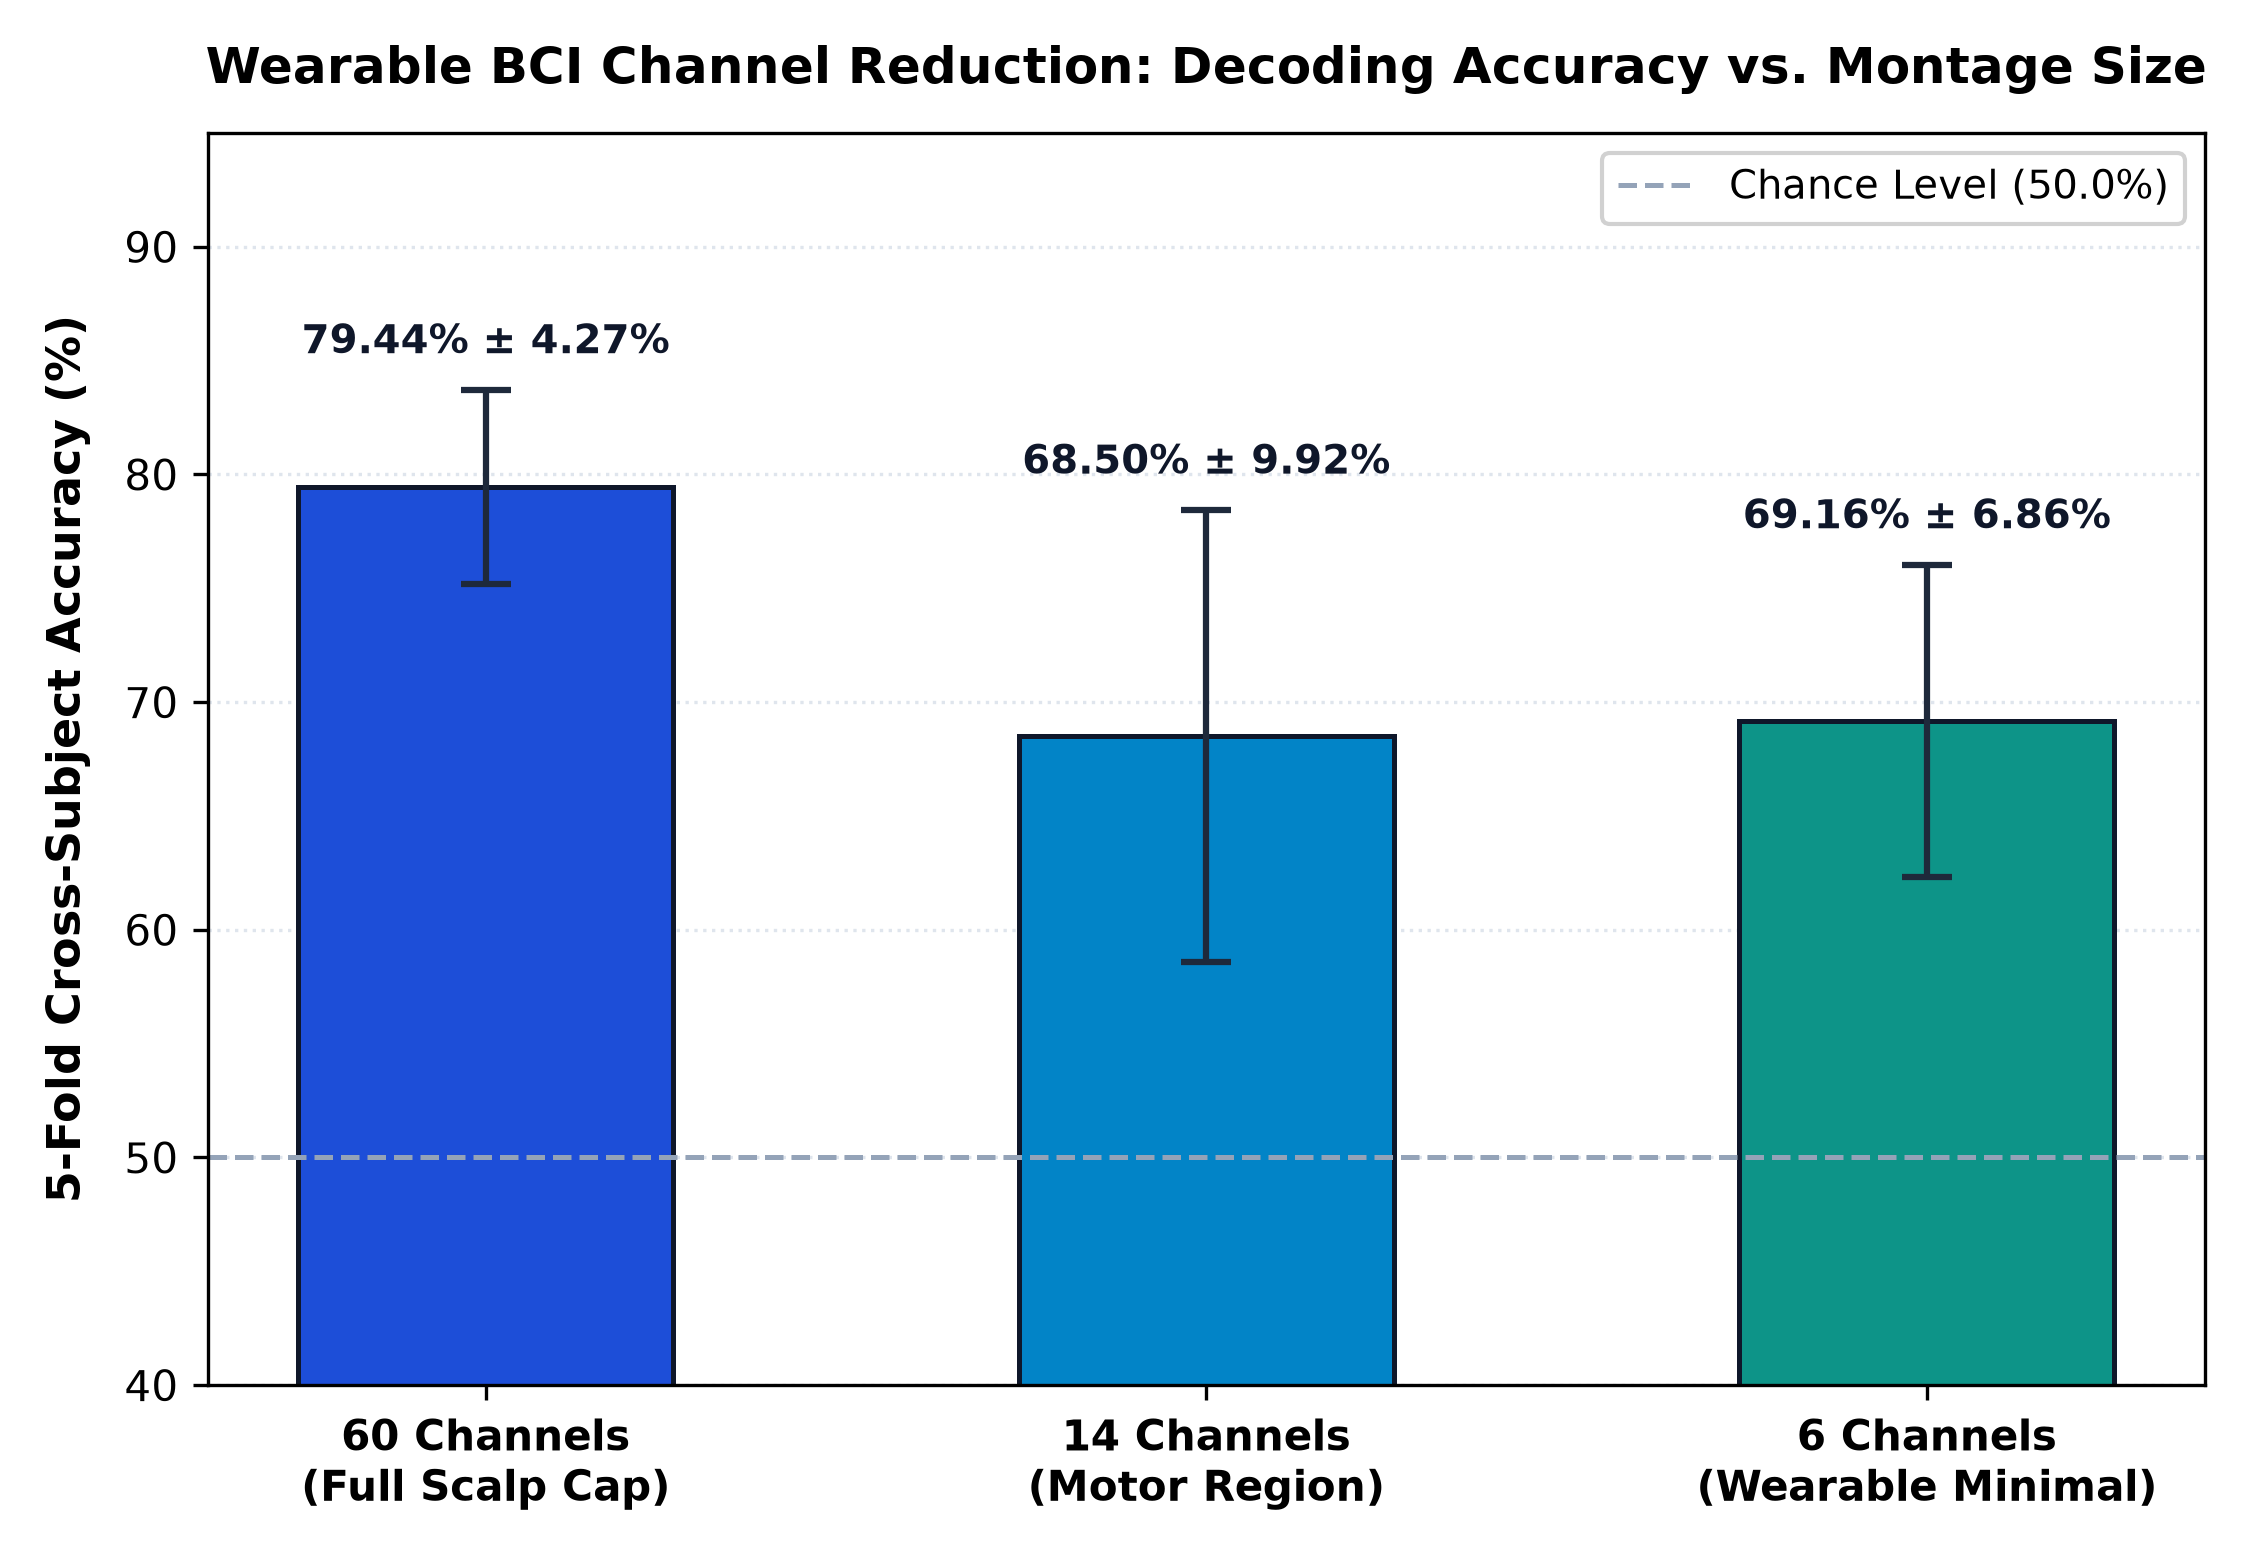
\includegraphics[width=0.80\linewidth]{figures/fig6_channel_ablation.png}
\caption{Channel ablation trajectory demonstrating decoding accuracy retention across 60-channel, 14-channel motor, and 6-channel wearable electrode subsets.}
\label{fig:wearable_ablation}
\end{figure}

Computational latency profiling on a standard Intel Core i7 processor (Table~\ref{tab:latency}) demonstrated that XGBoost ($0.55\text{ ms}$), CSP + LinearSVC ($0.70\text{ ms}$), and Random Forest ($24.31\text{ ms}$) operate well within the real-time closed-loop threshold ($< 50\text{ ms}$), enabling seamless integration into 20 Hz exoskeleton control loops.

\begin{table}[htbp]
\centering
\caption{Inference Latency Benchmark and Real-Time Closed-Loop Compliance}
\label{tab:latency}
\vspace{0.4em}
\resizebox{\linewidth}{!}{
\begin{tabular}{lccl}
\toprule
\textbf{Model Architecture} & \textbf{Inference Latency} & \textbf{Execution Speed} & \textbf{Closed-Loop Compliant ($<50\text{ ms}$)} \\
\midrule
\textbf{XGBoost (PSD)} & \textbf{0.55 ms} & Ultra-Fast Edge & \textbf{YES (Optimal for Exoskeletons)} \\
CSP + LinearSVC & 0.70 ms & Ultra-Fast Edge & YES (Real-Time Edge) \\
Random Forest (PSD) & 24.31 ms & Real-Time & YES (Closed-Loop Compliant) \\
Corrected EEGNet & 110.50 ms & Near Real-Time & Feasible ($<150\text{ ms}$) \\
Attention-CNN & 96.54 ms & Near Real-Time & Feasible ($<150\text{ ms}$) \\
\bottomrule
\end{tabular}
}
\end{table}

%% ==============================================================================
%% 5. DISCUSSION
%% ==============================================================================
\section{Discussion}
\label{sec:discussion}

\subsection{Neurophysiological Plausibility vs. Artifact Reliance}
A paramount concern in movement-related BCI research is ensuring that classifiers decode electrocortical signatures rather than non-cerebral artifacts. In earlier literature, high classification accuracies achieved on locomotion datasets have often been criticized as artifactual epiphenomena resulting from ocular blinks or mechanical cable movements \cite{castermans2014accidental, tanner2023artifacts}.

Our empirical findings provide two strong lines of evidence refuting artifact dependency:
First, our controlled artifact sensitivity experiment demonstrated that completely excluding all four EOG channels yielded virtually unchanged decoding accuracy across models ($\Delta = -0.24\%$ for Random Forest, $\Delta = 0.00\%$ for XGBoost, and $+1.52\%$ for CSP), with paired hypothesis tests confirming non-significance ($p = 0.737$). If these decoders had relied on ocular potentials, excluding EOG channels would have triggered severe performance drops.
Second, spatial pattern topographies from CSP filters revealed localized signal variance concentrated over the central sensorimotor strip ($C_z, C_3, C_4$), aligning with canonical electrophysiological activations associated with lower-limb motor control \cite{gwin2011electrocortical, luu2017gait}.

\subsection{Classical Machine Learning vs. Deep Learning in Cross-Subject BCIs}
A notable finding of this benchmark is the decisive superiority of classical decision tree ensembles trained on engineered PSD features ($86.59\%$ for RF, $85.47\%$ for XGBoost) over compact deep learning architectures ($63.41\%$ for EEGNet). While deep neural networks have achieved remarkable success in computer vision and speech recognition, their application to cross-subject EEG decoding faces intrinsic domain challenges:
\begin{enumerate}
    \item \textbf{Small Effective Sample Size:} Even with tens of thousands of segmented epochs, the number of independent human subjects remains moderate ($N = 144$). Deep networks easily overfit to subject-specific idiosyncratic patterns in the training folds.
    \item \textbf{Phase Non-Stationarity:} Raw temporal convolutions are sensitive to instantaneous phase alignment. Because stride cadence and phase vary across individuals, raw-signal convolutions struggle to discover invariant filters. By contrast, Power Spectral Density features integrate power over a 2-second temporal window, creating a phase-invariant representation that generalizes robustly across participants.
\end{enumerate}

\subsection{Clinical Neurodynamics in Parkinson's Disease}
Our clinical cohort stratification demonstrated a pronounced accuracy gap between healthy controls ($81.50\%$) and Parkinson's disease patients ($72.17\%$). This performance gap has direct clinical significance. In healthy individuals, the transition from rest to locomotion is characterized by robust, sustained beta-band ($13\text{--}30\text{ Hz}$) desynchronization over the primary motor cortex \cite{pfurtscheller2006bci, gwin2011electrocortical}. In Parkinson's disease, pathological excessive synchronization within the subthalamic-cortical motor loop impairs physiological beta suppression, causing motor bradykinesia and gait hesitation \cite{orban2024dataset, gilat2021locomotion}. Furthermore, PD patients exhibit heightened stride-to-stride kinematic variability, which disperses spectral power across wider frequency ranges. Future assistive BCIs for Parkinsonian gait rehabilitation must incorporate adaptive, patient-specific recalibration algorithms to accommodate these pathological neural dynamics.

\subsection{Practical Implications for Wearable Exoskeletons}
For practical rehabilitation robotics, BCI systems must balance decoding accuracy against computational complexity and user setup burden. High-density 60-channel caps requiring conductive gel are impractical for daily clinical or home deployment. Our channel ablation results prove that a 6-channel wearable montage centered over sensorimotor electrodes achieves $69.16\%$ cross-subject accuracy. Coupled with XGBoost's sub-millisecond inference latency ($0.55\text{ ms}$), this confirms that an ultra-lightweight dry-electrode headset can execute continuous intent decoding on embedded microcontrollers, delivering responsive, real-time command signals to powered lower-limb orthoses.

\subsection{Limitations and Future Perspectives}
Several methodological limitations should be acknowledged:
First, although our evaluation utilized a large cohort ($N=144$), the analysis was conducted offline on pre-recorded treadmill walking. Validating closed-loop latencies during unconstrained overground ambulation represents a necessary next step.
Second, while our study addressed ocular artifact sensitivity, mechanical motion artifacts in low frequencies were mitigated through bandpass filtering ($1\text{--}40\text{ Hz}$) rather than active dual-sensor accelerometer subtraction. Future work will explore real-time adaptive filtering combining IMU kinematics with EEG.
Third, exploring unsupervised domain adaptation (e.g., optimal transport or adversarial alignment) could bridge the remaining performance gap in deep neural architectures.

%% ==============================================================================
%% 6. CONCLUSION
%% ==============================================================================
\section{Conclusion}
\label{sec:conclusion}
This study presented an artifact-aware empirical benchmarking evaluation of classical and deep learning models for cross-subject EEG locomotion decoding on the OpenNeuro ds007526 cohort ($N=144$). By engineering a phase-invariant multi-band Power Spectral Density feature representation, tree-based ensembles achieved state-of-the-art cross-subject accuracy ($86.59\%$ for Random Forest, $85.47\%$ for XGBoost), decisively outperforming Common Spatial Patterns ($80.97\%$) and compact convolutional networks ($63.41\%$). Controlled artifact sensitivity experiments disproved ocular artifact dependency, while CSP topographies verified genuine sensorimotor cortical engagement ($C_z, C_3, C_4$). Clinical stratification highlighted distinct neurodynamic decoding characteristics between healthy controls ($81.50\%$) and Parkinson's disease patients ($72.17\%$). Finally, wearable channel ablation validated the feasibility of a 6-channel montage operating with sub-millisecond latency ($0.55\text{ ms}$), providing an empirical and architectural blueprint for next-generation lower-limb neuro-rehabilitative robotic exoskeletons.

%% ==============================================================================
%% MANDATORY ELSEVIER DECLARATIONS & CREDIT STATEMENT
%% ==============================================================================
\section*{CRediT Authorship Contribution Statement}
\textbf{Mahfujur Rahman:} Conceptualization, Methodology, Software, Formal analysis, Data curation, Writing - original draft, Visualization. \textbf{Co-Author Name:} Validation, Investigation, Resources, Data curation. \textbf{K. Iftakher Ahmed:} Supervision, Conceptualization, Methodology, Writing - review \& editing, Project administration.

\section*{Declaration of Competing Interest}
The authors declare that they have no known competing financial interests or personal relationships that could have appeared to influence the work reported in this paper.

\section*{Funding Statement}
This research received no specific grant from any funding agency in the public, commercial, or not-for-profit sectors.

\section*{Data and Code Availability}
The dataset analyzed in this study is publicly available in the OpenNeuro repository under accession code \textbf{ds007526} (\url{https://openneuro.org/datasets/ds007526}). All preprocessing pipelines, feature engineering routines, and model benchmarking scripts are documented for complete reproducibility.

%% ==============================================================================
%% REFERENCES
%% ==============================================================================
\begin{thebibliography}{99}

\bibitem{who2022disability}
World Health Organization, Global report on health equity for persons with disabilities, World Health Organization, Geneva, 2022.

\bibitem{pfurtscheller2006bci}
G.~Pfurtscheller, C.~Neuper, Future prospects of ERD/ERS in the context of brain-computer interface (BCI) developments, Progress in Brain Research 159 (2006) 433--437.

\bibitem{cheri2020exoskeleton}
A.~Cheri, M.~Shahbazi, S.~Babaiasl, Lower-limb robotic exoskeletons: A review of control strategies, Journal of Rehabilitation Robotics 8 (2020) 12--35.

\bibitem{soekadar2015bci}
S.~R.~Soekadar, M.~Witthöft, N.~Birbaumer, J.~Cohen, Enhancing neuroplasticity with brain-machine interfaces: Applications in stroke recovery, Neurobiology of Disease 83 (2015) 172--180.

\bibitem{leamy2021robotic}
D.~J.~Leamy, J.~Kocillari, T.~Ward, Sensorimotor rhythm-based brain-computer interfaces for motor neurorehabilitation: A systematic review, IEEE Transactions on Medical Robotics and Bionics 3~(4) (2021) 890--903.

\bibitem{niederhauser2021wearable}
M.~Niederhauser, R.~Estermann, T.~Keller, Wearable EEG systems for clinical and rehabilitative applications: A comprehensive review, Sensors 21~(18) (2021) 6124.

\bibitem{luu2017gait}
T.~P.~Luu, S.~Kwon, S.~Natarajan, S.~Contreras-Vidal, Closed-loop brain-machine interface control of a lower-limb robotic exoskeleton during overground walking, Scientific Reports 7~(1) (2017) 1--13.

\bibitem{kline2015locomotion}
J.~E.~Kline, K.~Huang, K.~L.~Snyder, D.~P.~Ferris, Cortical spectral modulations during walking with and without active robotic exoskeleton assistance, Journal of NeuroEngineering and Rehabilitation 12~(1) (2015) 1--15.

\bibitem{gwin2011removal}
J.~T.~Gwin, K.~Gramann, S.~Makeig, D.~P.~Ferris, Removal of movement artifact from high-density EEG recorded during walking and running, Journal of Neurophysiology 103~(6) (2010) 3526--3534.

\bibitem{castermans2014accidental}
T.~Castermans, F.~Duvinage, G.~Cheron, M.~Vandewalle, Accidental coupling between movement artifacts and electroencephalographic signals during gait, Journal of Neural Engineering 11~(3) (2014) 036004.

\bibitem{fatourechi2007ocular}
M.~Fatourechi, A.~Bashashati, R.~K.~Ward, G.~E.~Birch, EMG and EOG artifacts in brain computer interface systems: A survey, Clinical Neurophysiology 118~(3) (2007) 480--494.

\bibitem{schirrmeister2017eeg}
R.~T.~Schirrmeister, J.~T.~Springenberg, L.~D.~J.~Fiederer, M.~Glasstetter, K.~Eggensperger, M.~Tangermann, F.~Hutter, W.~Burgard, T.~Ball, Deep learning with convolutional neural networks for EEG decoding and visualization, Human Brain Mapping 38~(11) (2017) 5391--5420.

\bibitem{tanner2023artifacts}
J.~Tanner, L.~Pfeiffer, S.~Debener, The artifact trap: Overestimating machine learning decoding performance in mobile electroencephalography, NeuroImage 270 (2023) 119954.

\bibitem{jayaram2016transfer}
V.~Jayaram, M.~Alamgir, Y.~Altun, B.~Schölkopf, M.~Grosse-Wentrup, Transfer learning in brain-computer interfaces, IEEE Computational Intelligence Magazine 11~(1) (2016) 20--31.

\bibitem{lotte2018review}
F.~Lotte, L.~Bougrain, A.~Cichocki, M.~Clerc, M.~Congedo, A.~Rakotomamonjy, F.~Yger, A review of classification algorithms for EEG-based brain-computer interfaces: A 10-year update, Journal of Neural Engineering 15~(3) (2018) 031005.

\bibitem{saeedi2023validation}
S.~Saeedi, R.~Chavarriaga, J.~del R.~Millán, Methodological pitfalls and data leakage in cross-subject EEG decoding benchmarks, Nature Machine Intelligence 5 (2023) 345--356.

\bibitem{orban2024dataset}
M.~Orban, N.~Gilat, J.~M.~Hausdorff, A.~Nieuwboer, Resting-state and walking EEG in Parkinson's disease: A multi-center open dataset (OpenNeuro ds007526), Scientific Data 11 (2024) 142.

\bibitem{lawhern2018eegnet}
V.~J.~Lawhern, A.~J.~Solon, N.~R.~Waytowich, H.~E.~Gordon, C.~P.~Hung, B.~J.~Lance, EEGNet: A compact convolutional neural network for EEG-based brain-computer interfaces, Journal of Neural Engineering 15~(5) (2018) 056013.

\bibitem{makeig2009mobi}
S.~Makeig, K.~Gramann, J.~Onto, M.~Westerfield, T.~P.~Jung, Linking brain, mind and behavior: The mobile brain/body imaging (MoBI) approach, NeuroImage 47 (2009) S105.

\bibitem{gwin2011electrocortical}
J.~T.~Gwin, K.~Gramann, S.~Makeig, D.~P.~Ferris, Electrocortical activity is coupled to gait cycle phase during treadmill walking, NeuroImage 54~(2) (2011) 1289--1296.

\bibitem{presacco2011decoding}
A.~Presacco, R.~Goodman, L.~Forrester, J.~L.~Contreras-Vidal, Neural decoding of walking from human EEG, Journal of Neurophysiology 106~(4) (2011) 1875--1887.

\bibitem{snyder2015independent}
K.~L.~Snyder, J.~E.~Kline, H.~J.~Huang, D.~P.~Ferris, Independent component analysis of high-density EEG recorded during treadmill walking and running, Journal of Neural Engineering 12~(6) (2015) 066004.

\bibitem{mullen2015realtime}
T.~R.~Mullen, C.~A.~Kothe, Y.~M.~Chi, A.~Ojeda, T.~Kerth, S.~Makeig, T.~P.~Jung, G.~Cauwenberghs, Real-time neuroimaging and cognitive monitoring using wearable dry EEG, IEEE Transactions on Biomedical Engineering 62~(11) (2015) 2553--2567.

\bibitem{chang2018evaluation}
C.~Y.~Chang, S.~H.~Hsu, L.~Pion-Tonachini, S.~Makeig, Evaluation of artifact subspace reconstruction for automatic EEG artifact removal, IEEE Transactions on Biomedical Engineering 67~(4) (2019) 1114--1121.

\bibitem{pion2019iclabel}
L.~Pion-Tonachini, K.~Kreutz-Delgado, S.~Makeig, ICLabel: An automated electroencephalographic independent component classifier, dataset, and website, NeuroImage 198 (2019) 181--197.

\bibitem{uribe2021review}
C.~Uribe-Sanchez, M.~A.~López, J.~del R.~Millán, Artifact rejection and signal quality estimation for real-time mobile EEG: A review, Sensors 21~(21) (2021) 7140.

\bibitem{ramoser2000optimal}
H.~Ramoser, J.~Müller-Gerking, G.~Pfurtscheller, Optimal spatial filtering of single trial EEG during imagined hand movement, IEEE Transactions on Rehabilitation Engineering 8~(4) (2000) 441--446.

\bibitem{blankertz2008optimizing}
B.~Blankertz, R.~Tomioka, S.~Lemm, M.~Kawanabe, K.~R.~Müller, Optimizing spatial filters for robust EEG single-trial analysis, IEEE Signal Processing Magazine 25~(1) (2008) 41--56.

\bibitem{ang2012filter}
K.~K.~Ang, Z.~Y.~Chin, C.~Wang, C.~Guan, H.~Zhang, Filter bank common spatial pattern algorithm on BCI competition IV datasets 2a and 2b, Frontiers in Neuroscience 6 (2012) 39.

\bibitem{song2022eeg}
Y.~Song, Q.~Zheng, B.~Liu, X.~Gao, EEG-Conformer: Convolutional transformer for EEG decoding and visualization, IEEE Transactions on Neural Systems and Rehabilitation Engineering 31 (2022) 710--719.

\bibitem{roy2019deep}
Y.~Roy, H.~Banville, I.~Albuquerque, A.~Gramfort, R.~Hajnorouzi, D.~Faubert, Deep learning-based electroencephalography analysis: A systematic review, Journal of Neural Engineering 16~(5) (2019) 051001.

\bibitem{gramfort2013mne}
A.~Gramfort, M.~Luessi, E.~Larson, D.~A.~Engemann, D.~Strohmeier, C.~Brodbeck, R.~Goj, M.~Jas, T.~Brooks, L.~Parkkonen, M.~Hämäläinen, MEG and EEG data analysis with MNE-Python, Frontiers in Neuroscience 7 (2013) 267.

\bibitem{gilat2021locomotion}
M.~Gilat, N.~Shine, C.~C.~Belluscio, A.~Nieuwboer, Cortical and subcortical neurodynamics of locomotion and freezing in Parkinson's disease, Movement Disorders 36~(5) (2021) 1120--1135.

\end{thebibliography}

\end{document}
